\documentclass[a4paper]{article}

%% Language and font encodings
\usepackage[french]{babel}
\usepackage[utf8x]{inputenc}
\usepackage[T1]{fontenc}

%% Sets page size and margins
\usepackage[a4paper,top=3cm,bottom=2cm,left=3cm,right=3cm,marginparwidth=1.75cm]{geometry}

%% Useful packages
\usepackage{siunitx}
\usepackage{amsmath}
\usepackage{graphicx}
\usepackage{amssymb}
\usepackage[colorinlistoftodos]{todonotes}
\usepackage[colorlinks=true, allcolors=blue]{hyperref}

\graphicspath : \graphicspath{{Images/}}

\title{Réflexion et différent essai du rendu d'ombre et de sa colorisation.}
\author{Jonathan Granier}

\begin{document}
\maketitle



\section{Toon Shading - Cell Shading}
\subsection{Principe}
Faire une apparence cartoon avec des aplats de couleur (ex : windwaker). On calcule l'intensité de la lumière en chaque point , en fonction de l'intensité on sélectionne la couleur du point dans une texture 1D. Classiquement la texture est un dégradé ou alors une succession d’aplat de couleur.   
\[Intensity = lightVector . normalVector \]



\subsection{Limites - Inconvénients}
\begin{itemize}
\item Indépendant du point de vue.
\item Ne prend pas en compte le niveau d'abstraction
\item La moindre petite aspérité va être rendu avec le maximum de précision.  
\end{itemize}




\section{xToon - Toon shading 2D}
\subsection{Principe}
Essaye de corriger les problème du toon shading 1D en rajoutant une deuxième dimension à la texture. 
La sélection de la couleur se fait en fonction de l'intensité  et aussi d'un paramètre D. \\ 

\[Intensity = lightVector . normalVector \]

\begin{center}
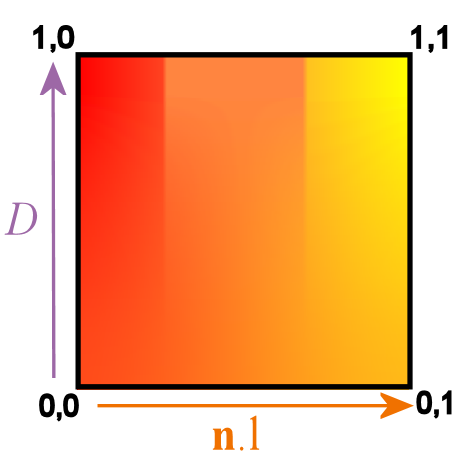
\includegraphics[scale=0.2]{xToon.png}
\end{center}


\subsection{Limites - Inconvénients}
\begin{itemize}
\item Trouver D.
\item Trouver la texture.
\item Aspect très cartoon
\end{itemize}


\section{Exaggerated Shading}
\subsection{Principe}
Shading non réaliste pour exagérer les ombres afin d'avoir une meilleur perception des aspérités d'une surface.  
Le principe est de modifier localement la normal et avec ceci calculer un nouveau vecteur lumière. 

\[c = \frac{1}{2}+ \frac{1}{2}  * \left( k_b ( n_b\dot{l_{global}}) + \sum_{i=0}^{b-1}k_i c_i \right)\]
Avec : \\
\begin{itemize}
\item $c$ : la couleur du pixel
\item $l_{global}$ : le vector lumière venant du point de lumière de la scène.
\item $b$ : le nombre de passe pour lisser les normals.
\item $k$ : a constant
\item $c_{i} = clamp a(n_i\dot{l_{i+1}})$
\item $l_{i+1} = l_{global} - n_{i+1}(n_{i+1}\dot{l_{global}}) $
\item $n_{i+1}$ : La normal lisser par rapport aux normals l'entourant.
\end{itemize}


Voir si il ne travaille que avec l'élévation. 


\subsection{Limites - Inconvénients}
\begin{itemize}
\item Aspect bas relief , on semble perdre la notion de "GRAND" relief. 
\item Changement local , pas de contrôle sur une lumière global.
\end{itemize}




% Jap 1
\section{Stylized lighting for cartoon shader}
\subsection{Principe}
Faire un cel shading plus continue et homogène. Ne pas avoir de changement brut entre une face et celle d'à côté.  
On à un ensemble de couleur uniform (Typical toon shading). Pour chaque couleur , on définie une limite basse et haute à partir de la lumière diffuse d'un point de la surface arbitraire. On appelle cet ensemble D. 
\[ D_i := {p \in S | \delta_{i-1} \leq I_d(p) < \delta_i} (i=1,2,...,m)\]
Ensuite il bidouille la normal et la lumière de manière local. 



\subsection{Limites - Inconvénients}
\begin{itemize}
\item A quel point ça nous intéresse ?  
\item Ne prend pas en compte les ombres (futurwork). 
\item c'est compliqué avec pas mal de paramètre (la définition des limites peut se faire de plein de manière différente).
\end{itemize}

% Jap 2
\section{Locally Controllable Stylized Shading}
\subsection{Principe}
Faire une contrôle local d'un cel shading.\\ 
C'est compliqué...

\subsection{Limites - Inconvénients}
Utilisable seulement dans un logiciel de retouche d'objet. Pas de méthode général. 



% Test pour savoir le meilleur angle
\section{The assumed light direction for perceiving shape from shading}
\subsection{Principe}
Une étude de la perception du relief d'un objet en fonction de l'angle sur des utilisateurs.\\
On place une lumière en arc de cercle derrière la camera d'un angle allant de $-66\%$ à $+66\%$.
Conclusion : on la perception est meilleur quand la lumière se trouve à $+22\%$ au dessus de la camera.  


\begin{center}
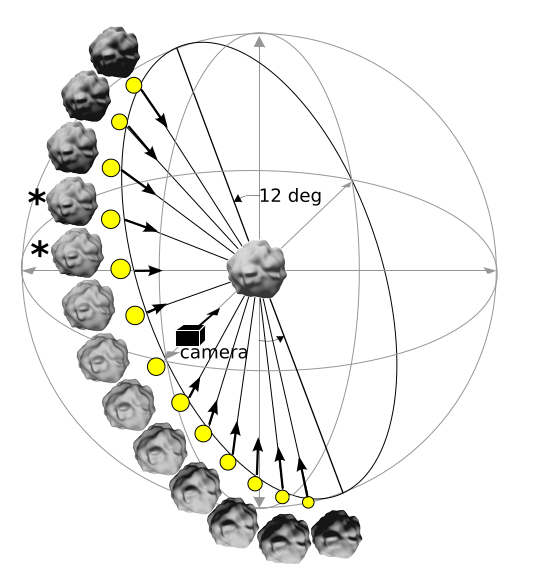
\includegraphics[scale=0.5]{LightDirection.png}
\end{center}

\subsection{Limites - Inconvénients}
Est-ce que c'est exploitable dans notre cas?


% Base 
\section{Shading de Vincent}
\subsection{Principe}
Avoir un éclairage non conventionnel avec une lumière défini en chaque point qui est soit à droite , soit à gauche de la camera. 
\\
Soit : \\
\begin{itemize}
\item $p$ la position du point du monde actuel.
\item $c$ la position de la camera
\item $\vec{cd}$ la direction de la camera (attention elle ne correspond à $p-c$
\item $\vec{cu}$ la vertical de la camera dans l'espace : (est-ce qu'elle correspond bien à la perpendiculaire à cameraDir ?) 
\end{itemize}  






\[ \vec{cp} = p - c\]
\[ p' = p - \vec{cp} \cdot{\vec{cu}} * \vec{cu}\]
\[ \vec{cp'} = normalize(p' - c) \]
\[ cos\theta = \vec{cp'} \cdot{\vec{cd}}\] 
\[ parabole = 2.0 \]
\[ N0 = \frac{parabole}{(1.0 - cos\theta)} * \vec{cp'}\]
\[\vec{zplane} = \vec{cd} \times \vec{cu}\]
\[x = N0\cdot{\vec{zplane}}\]
\[\vec{lv} = \frac{\pm\sqrt{2.0*parabole}}{2.0*\sqrt{\pm x}} * \vec{zplane} + \vec{cd} - 0.3* \vec{cu} \]
\[\vec{lv} = normalize(\vec{lv})\]
\[ -\vec{lv} \cdot \vec{normal}\]




La fonction parabola construit une fonction en Y en fonction X (X et Y coordonnée de l'écran). 
On a trouvé une autre formule mais il faudrait la généralisé 
Soit $y$ le facteur de $\vec3{zplane}$ : 
\[ y = \pm \frac{1}{\sqrt{\left| \frac{\frac{-|x|}{x} . \frac{\ln(|x|+1)}{65} - \frac{1}{x}}{3,7.10^{-4}} \right|}}\]
Avec $x\in [-6,6]$.

En faite : Le seul élément Pifé par Vincent est l'élément le plus important 


Conclusion : 

Directional :
\[\alpha = \frac{\pi}{2} * \frac{angle}{10}\]
\[\vec{lv} =  
\begin{pmatrix}
\vec{cd}_x \\
0 \\
\vec{cd}_z \\
\end{pmatrix} *
\begin{pmatrix}
\cos\alpha & 0 & \sin-\alpha \\
0 & 0 & 0 \\
-\sin-\alpha & 0 & \cos\alpha 
\end{pmatrix}\]

\[\vec{lv} = normalize(\vec{lv}) / 2.0 \]
\[ D = -\vec{lv} \cdot{\vec{normal}} \]


\subsection{Limites - Inconvénients} 
Très hard-codé \\
Ne respect pas vraiment le coté gauche droite.  \\
A retravailler. \\



\section{Apparent relief: a shape descriptor for stylized shading}
\subsection{Principe}
A partir d'un object , on extrait une forme décrite par un code couleur.
Et a partir de ce code couleur , on créer un ombrage. 

\begin{center}
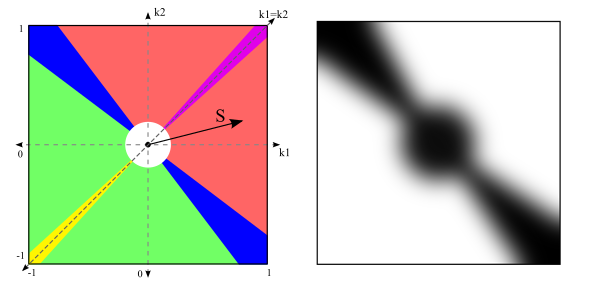
\includegraphics[scale=0.5]{Shape_descriptor.png}
\end{center}

Les axes $k1$ et $k2$ correspondent au principal courbures de l'objet et le vecteur $\vec{S}$ représente le vecteur de forme d'un point , avec la direction $\vec{D}$ qui représente ça convexité et sa longueur $\vec{L}$ qui représente sa courbure.\\
On calcule $\vec{D}$ dans l'espace objet et $\vec{L}$ dans l'espace image. 
$\vec{D}$ est calculé avec la méthode (1)
On applique un flou gaussien sur k1 et k2 
\[k_1^*(x,y) = k_2(x,y) \ast  g(x,y,\sigma)\]
\[k_2^*(x,y) = k_2(x,y) \ast  g(x,y,\sigma)\]
Puis on calcul $\vec{D}$ 
Ensuite pour calculer $\vec{L}$ ,on part des normals $n_1$ et $n_2$ auquel on applique une gaussien : 
\[\nabla n_1 (x,y) = 
\begin{pmatrix}
n_1(x,y) \ast  g_x(x,y,\sigma) \\
n_1(x,y) \ast  g_y(x,y,\sigma) \\
\end{pmatrix}\] 
\[\nabla n_2 (x,y) = 
\begin{pmatrix}
n_2(x,y) \ast  g_x(x,y,\sigma) \\
n_2(x,y) \ast  g_y(x,y,\sigma) \\
\end{pmatrix} 
\]
Ensuite on calcule le gradient direction dans l'espace vectoriel : 
\[\nabla n_x = 
\begin{pmatrix}
\nabla n_1 \cdot{x} \\
\nabla n_2 \cdot{x} \\
\end{pmatrix}\] 
\[\nabla n_y = 
\begin{pmatrix}
\nabla n_1 \cdot{y} \\
\nabla n_2 \cdot{y} \\
\end{pmatrix}\] 

Puis on calcule le champ tensoriel symétrique :
\[N = 
\begin{pmatrix}
N_{11} & N_{12} \\
N_{21} & N_{22} \\
\end{pmatrix}= 
\begin{pmatrix}
\nabla n_x \cdot{\nabla n_x} & \nabla n_x \cdot{\nabla n_y}\\
\nabla n_y \cdot{\nabla n_x} & \nabla n_y \cdot{\nabla n_y}\\
\end{pmatrix}\] 

$\vec{L}$ est le maximum de $N$.
Enfin $\vec{S} = \vec{D}\dot{\vec{L}} $
Et utilise $\vec{S}$ comme une coordonnée de texture tout simplement. 
\subsection{Limites - Inconvénients}

\subsection{Listes des papiers annexe}
(1) Estimating Curvatures and Their Derivatives on Triangle Meshes
\section{Perceptually-motivated shape exaggeration}
\subsection{Principe}

\subsection{Limites - Inconvénients}



\section{Making 3D Terrain maps}
\subsection{Principe}
C'est un tuto de comment faire des cartes bien.
Élément intéressante sur la lumière :
\begin{itemize}
\item Parfois les ombres porté empêche une bonne lecture du terrain , ne pas en mettre de partout
\item Orientation : Pour une map orienté plein nord , c'est soit sud-est (135) ou sud ouest (225) ($\pm 30$)
\item Hauteur : 20 à 50 sur l'horizon.
\item $25\%$ à $50 \%$ de lumière ambiante.
\item On ajoute plusieurs lumière pour rajouter des ombres et donc améliorer la lecture.
\item assombrir le $1^{er}$ plan qui est inintéressante. 
\item Rajouter du brouillard au fond 
\end{itemize}

\begin{center}
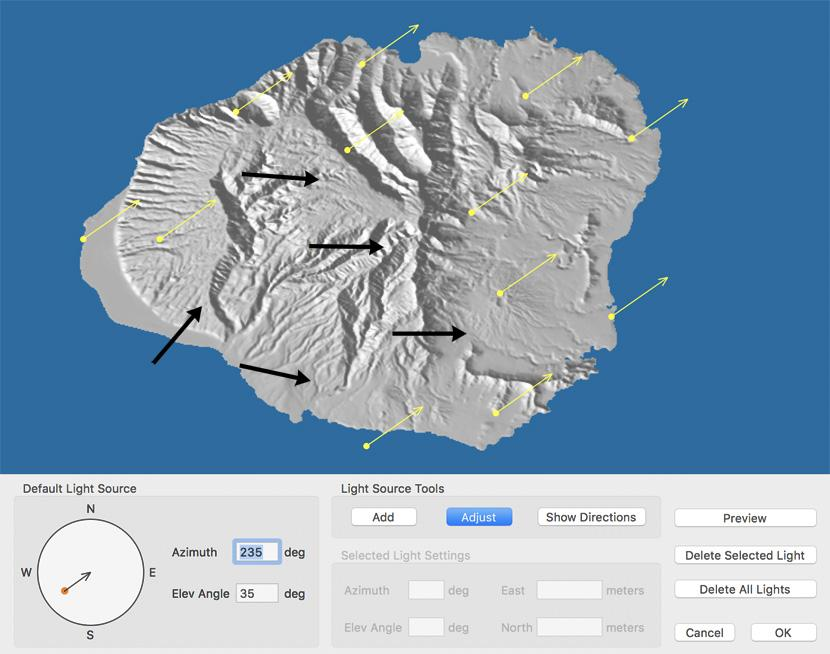
\includegraphics[scale=0.5]{multiple_light.jpeg}
\end{center}


\subsection{Limites - Inconvénients}
C'est un tuto pour faire des cartes.


\section{Creating value-enhanced shaded relief in Photoshop}
\subsection{Principe}
Tutoriel pour avoir à la fois le détail d'une carte et un haut niveau de contraste. 
La solution est de générer 2 ombrage de la carte : Une avec exagération vertical à 1 (normal) pour les contrastes et une autre à une exagération vertical à 0.25 pour avoir plus de détails et ensuite de les fusionner pour garder le meilleur de chaque ombrage.   

\subsection{Limites - Inconvénients}
C'est un tuto pour faire des cartes.

\section{Relief Shading - Design }
\subsection{Principe}
Explique comment faire un shading de montagne vu de dessus à la main. 
L'éclairage Nord Ouest est meilleurs pour la lecture que l'éclairage sud-est. \\
En général , on place la lumière à $45°$ mais on peut ajuste pour certain endroit particulier. \\
Les grandes formes de relief montrent la configuration globale de la topographie et les reliefs plus petites contiennent plus de détail unique et apporte du caractère à un relief ombragé. \\
Les zone plate au fond des montagnes doivent être légèrement plus sombre que les zone plate en haut de montagnes afin d'avoir un meilleur effet de relief. \\
Les objets au premier plan sont plus contrasté et les objets en arrière plan sont plus lumineux et moins contrasté. \\
Logiquement : plus on est loin , moins on met de détail dans la montagne et l'ombrage. \\ 



\subsection{Limites - Inconvénients}
C'est un tuto pour faire des cartes.\\
C'est pensé pour faire des cartes vu de dessus et sans déformation. 


\section{Relief Shading - Analytical }
\subsection{Principe}
Explique comment le shading est fait de manière automatique grâce à un ordinateur. 
Model d'illumination local proposé par l'auteur : Diffuse reflection, Phong model, Bliin reflection, Lommel-Seeliger Law, Minnaert's reflectance function. 

Proposition d'une methode d'illumination : 
\[gray value = \cos\alpha + 12 \]
avec $\alpha$ l'angle entre l'aspect et l'azimut de la direction de la lumière.
La solution proposé est d'utiliser une combinaison entre le diffus et l'aspect avec ce rapport : 
threshold
\begin{center}
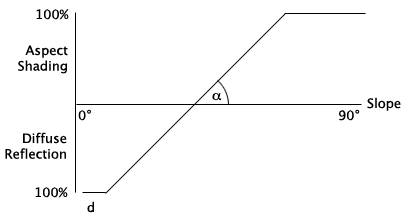
\includegraphics[scale=0.5]{diagram_diffuse_aspect.png}
\end{center}

Solution pour les zone plates :\\
Généralement les zone plates sont trop grise donc il propose d'utiliser une moyenne pondérer :
\[ g' = w.g + (1-w) .f \]
Avec :
\begin{itemize}
\item $g'$ Le nouveau ton de gris
\item $g$ le ton de gris initial
\item $f$ le ton de gris voulu pour une zone plate. 
\item $w$ le poids de l'ombrage.
\end{itemize}

Et $w$ peut être calculé avec 
\[if s > a : w = e^{\ln\frac{s-a}{90-a} x b} else : w = 0\]
Avec : 
\begin{itemize}
\item $s$ Pente du point (en degrés). 
\item $a$ la pente maximum sans shading. 
\item $b$ Courbure $[0..1]$. 
\item $w$ le poids de l'ombrage.
\end{itemize}



Ils font des ajustement local de la lumière quand la montagne est mal orienté par rapport au soleil. 

\subsection{Limites - Inconvénients}
Assez simpliste.


\section{Fast and Robust Detection of Crest Lines on Meshes}
\subsection{Principe}
Faire une détection des crêtes d'un maillage. Avec un paramètre T pour définir une limite.  
2 parties : \\
\subsubsection{Détection des crêtes}
On prend un maillage $M$\\
Pour chaque vertex $p \in M$ , on créer un nouveau $p'$ dans un maillage $M'$ , où $p'$ est le vertex $p$ mais lissé grâce au centroïde des triangles voisins. (Il doit avoir un algo simple).\\
Ensuite pour chaque $p' \in M'$, on recalcule sa normal (1) \\

Enfin pour chaque $p'$ et un ensemble de vertex connexe d'une distance $k$ (1,2,3 ou 4 en pratique) auquel on supprime les vertex $v$ dont l'angle de la normal de $v$ est $> 90$ avec la normal de $p'$, on applique ce polynôme cubique (2): 
\[h(x,y) = \frac{1}{2} (b_0x^2+2b_1xy+b_2y^2) + \frac{1}{6} (c_0x^3 + 3c_1x^2y+3c_2xy^2 + c_3y^3) \] 
"Then a cubic polynomial is fitted in the least-square sense to $p'$ and his set. Next the curvature tensor and extremality coefficients are expressed via derivatives of local cubic polynomial h(x, y)." \\
J'ai pas compris comment ça marche et comment on l'utilise. 

Et pour finir on ajoute ces attributs de courbures au vertex original $p$

\subsubsection{Traçage et seuillage des lignes de crêtes}
Pour chaque sommet de $M$ , on regarde s'il contienne une courbure maximal ou minimal. Si c'est le cas on connecte les sommets entre eux avec la procédure de Ohtake (3). 
Ensuite pour réduire la fragmentation, pour chaque vertex on regarde les vertex en anneau (de taille 1) autour de lui et on regarde si on peut relier son point final à un point final d'un autre vertex voisins (s'il existe) . \\
On le fait si $\alpha \leq \frac{\pi}{3}$ , $\beta \leq \frac{\pi}{3}$,  $\gamma \leq \frac{\pi}{2}$.


\begin{center}
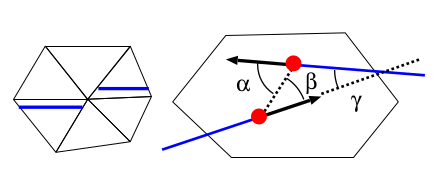
\includegraphics[scale=0.5]{Crest_detection.png}
\end{center}

Ensuite pour le seuil , j'ai pas compris comment ça marchais. 



\subsubsection{Listes des papiers annexe}

(1) Weights for Computing Vertex Normals from Facet Normals\\
(2) A Novel Cubic-Order Algorithm for Approximating Principal Direction Vectors \\
(3) Ridge-Valley Lines on Meshes via Implicit Surface Fitting
\subsection{Limites - Inconvénients}
Comment l'utiliser ?
Quel limite choisir ? 
Est-ce que ça fonctionnerai bien pour faire du placement de lumière. 


\section{Structure-aware Stylization of Mountainous Terrains}
\subsection{Principe}
La partie qui nous interresse est la dectection de la structure de la montagne
D'abord il fond une detection de crete (avec la méthode vue juste avant) et applique un seuil différent en fonction du niveau de détail (3,5,12,16), plus le seuil est haut , moins il a de crête. 




\subsection{Limites - Inconvenients}
C'est pour des mesh en 3D, on peut faire plus simple avec la carte de hauteur. 



\section{Paralaxe mapping}   
\subsection{Principe}
A partir d'une carte de hauteur et d'un vecteur lumière on peut savoir si un pixel est dans l'ombre ou non. 

\subsection{Source}
\url{https://en.wikipedia.org/wiki/Parallax_mapping}\\
\url{http://www.iquilezles.org/www/articles/terrainmarching/terrainmarching.htm}\\
\url{http://sunandblackcat.com/tipFullView.php?l=eng&topicid=28}\\

\section{Curvature Romain}

A partir d'une texture de normal où $n$ est la normal 3D à la position $x,y$ de la texture

hessianMatrix :

\[H = normal(x,y)  \circledast (Gradiant(n).G(x,y,\sigma)) \]
avec
\[Gradiant(n) = d * 
\begin{pmatrix}
n_{x} \\
n_{y} \\
\end{pmatrix}\] 
ou f est 
\begin{align*}
d &= \frac{-1}{1*(1-f)+f*z} \\
  &= \frac{-1}{f*(z-1) +1}
\end{align*}
avec $f = [0,1]$

Donc on se retrouve avec cette matrice qui est la dérivé de la normale : 
\[H = 
\begin{pmatrix}
\partial_{xx} & \partial_{xy} \\
\partial_{yx} & \partial_{yy} \\
\end{pmatrix}\] 

Or $\partial_{xy} = \partial_{yx}$ Donc

\[H = 
\begin{pmatrix}
\partial_{xx} & \partial_{xy} \\
\partial_{xy} & \partial_{yy} \\
\end{pmatrix}\] 

Propriété de H :

\[\left\{
    \begin{array}{ll}
        \mbox{Convexe en x } & \mbox{si } \partial_{xx} > 0 \\
       	\mbox{Concave en x } & \mbox{si } \partial_{xx} < 0 \\
       	\mbox{Convexe en y } & \mbox{si } \partial_{yy} > 0 \\
        \mbox{Concave en y } & \mbox{si }  \partial_{yy} < 0 \\
        \mbox{En Selle en } x,y & \mbox{si }  \partial_{xy} > 0 \\
		\mbox{En Selle en } x,-y & \mbox{si } \partial_{xy} < 0 \\
		\mbox{Plat} & \mbox{sinon}				
    \end{array}
\right.
\]
\\

Ensuite on calcule les valeurs propres:

\[ \Delta = \sqrt{(\partial_{xx} - \partial_{yy})^2 + 4\partial_{xy}^2} \]
\[ \lambda_1 = \frac{1}{2} * (\partial_{xx}+\partial_{yy} + \Delta) \]
\[ \lambda_2 = \frac{1}{2} * (\partial_{xx}+\partial_{yy} - \Delta) \]
\[\vec{e_1} = 
\begin{pmatrix}
\partial_{xy} \\
\lambda_1 - \partial_{xx} \\
\end{pmatrix}\] 
\[\vec{e_2} = 
\begin{pmatrix}
\lambda_1 - \partial_{xx} \\
-\partial_{xy} \\
\end{pmatrix}\] 


Pour la suite on considère que $\lambda_1 \geq \lambda_2$  et donc par consequence , $\vec{e_1}$ est le vecteur de courbure max du point. 

Avec cette courbure, on calcule le vecteur lumière. 

Notre objectif est de calculer un vecteur lumière local a partir de la courbure du point et du vecteur de lumière global. 


Soit le vecteur 3D de lumière global $\vec{L}$ définie par ses angles d'euler $\alpha$ et $\gamma$ : 

\[
\vec{L} = 
\begin{pmatrix}
X \\
Y \\
Z \\
\end{pmatrix}
=
\begin{pmatrix}
\cos \gamma  \cos \alpha\\
\sin \gamma \\
\cos \gamma  \sin \alpha \\
\end{pmatrix}
\] 

On définie  le vecteur 2D $\vec{l}$ la projection de $\vec{L}$ sur le plan $xz$ tel que :
\[\vec{l} =  
\begin{pmatrix}
\vec{L_x} \\
\vec{L_z} \\
\end{pmatrix}\]


On part du principe que tout les vecteurs sont normalisé. 


Liste des discontinuité 
\begin{itemize}

\item Quand la lumière est perpendiculaire à la courbure.
\item Quand c'est isotopique.
\item Quand la curvauture max n'est pas aligner avec la normal.
\item Une autre qui apparait que lorsqu'on ajoute le bruit de perlin. 	

\end{itemize}


\subsection{Phong}



\begin{figure}[thb]
	\centering
    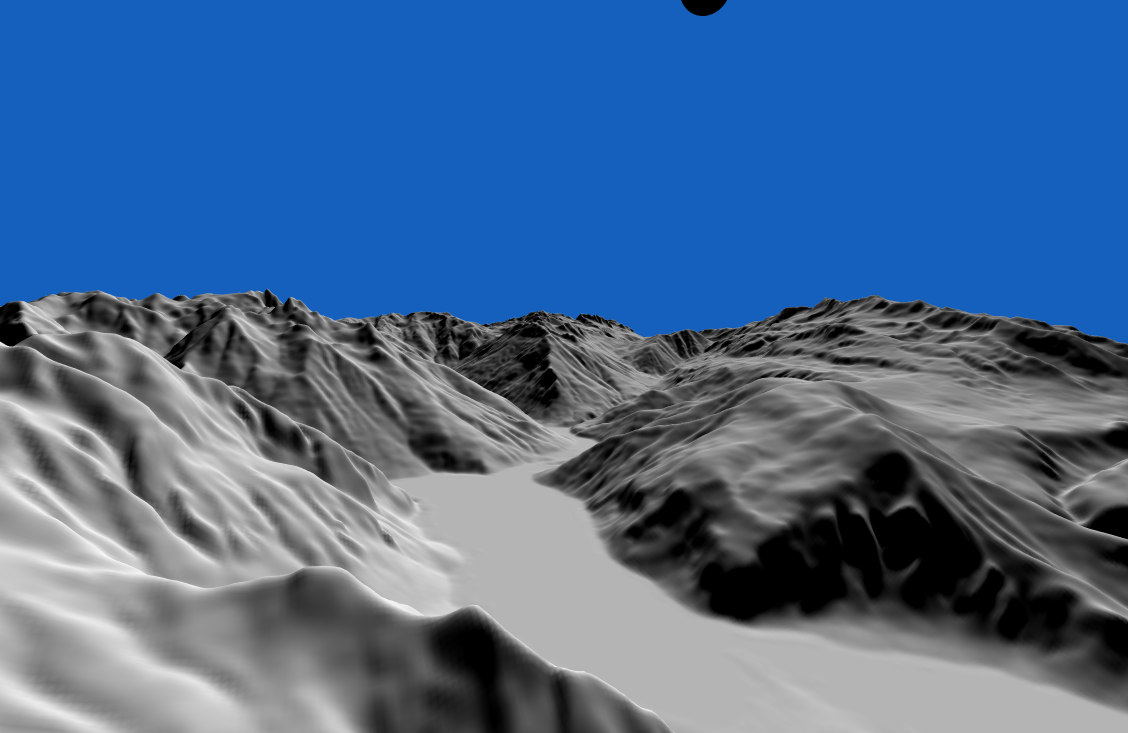
\includegraphics[scale=0.3]{Images/Essais/phong_mount.png}
    \caption{"Les montagnes avec uniquement un diffus"}
 \end{figure}



\begin{figure}[thb]
	\centering
    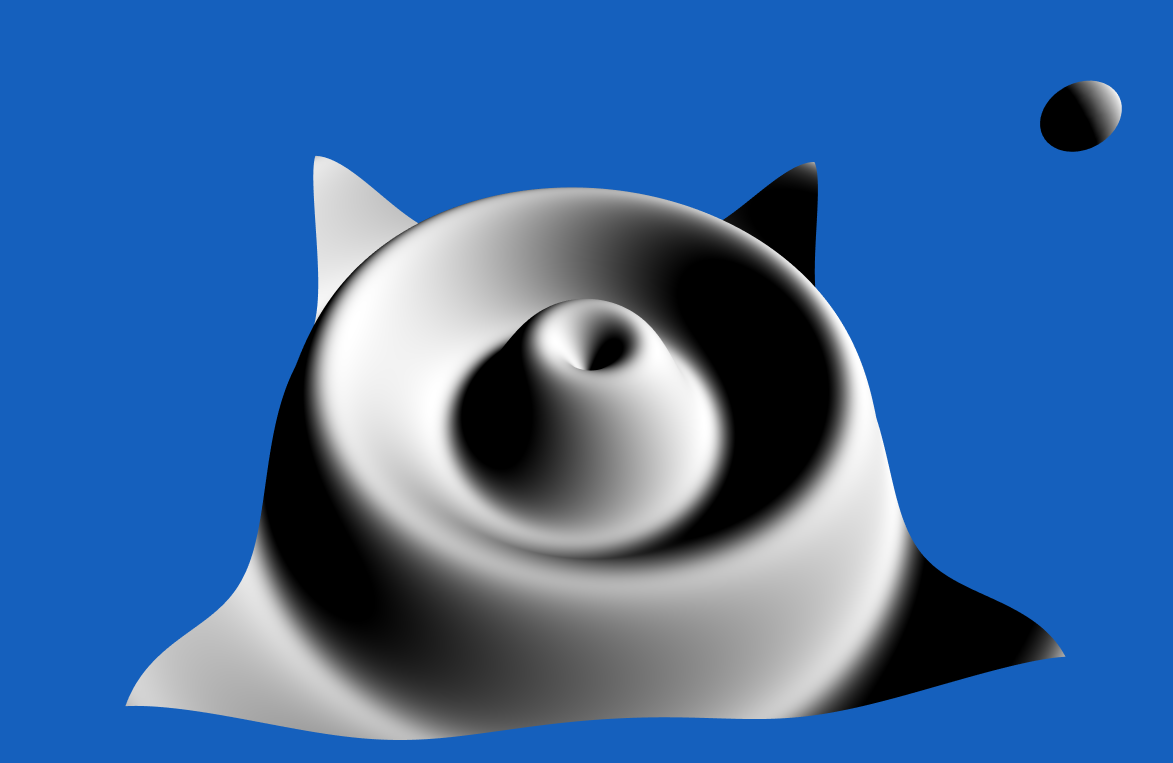
\includegraphics[scale=0.3]{Images/Essais/phong_toy.png}
    \caption{"Le jouet avec uniquement un diffus "}
 \end{figure}


\subsection{Essaie 1}

\subsubsection{Principe}
Pour ce 1er essaie , on aligne bêtement la lumière avec la courbure.
Donc dans un $1^{er}$ on souhaite a ne pas retourner complement notre vecteur lumière . Ça veut dire qu'on veut que l'angle de correction soit dans l'intervalle  $-\frac{\pi}{2}$ et $\frac{\pi}{2}$ . Ainsi si $\vec{l} \cdot{\vec{e_1}} < 0 $ alors on retourne $\vec{e_1} $


\[ \vec{e_1} = 
\left\{
    \begin{array}{ll}
        -\vec{e_1} & \mbox{si } \vec{l} \cdot{\vec{e_1}} < 0 \\
		\vec{e_1}  & \mbox{sinon}				
    \end{array}
\right.
\]

Ensuite on calcule l'angle $\theta$ entre $\vec{l}$ et $\vec{e_1}$ :
\[ \theta =  \arccos( \vec{l} \cdot{\vec{e_1}}) \]
Ici $\theta$ est dans l'intervalle  $[0,\frac{\pi}{2}]$ on le signe avec le determinant $\Delta$ pour qu'il soit dans l'intervalle $-\frac{\pi}{2}$ et $\frac{\pi}{2}$ :
\[\Delta =  \vec{l_x}\vec{e_{1_y}} - \vec{l_y}\vec{e_{1_x}}\]
\[\theta = \frac{\Delta}{|\Delta|}  \theta\]


Ensuite on applique un facteur à $\theta$   soit $S$ l'index de forme (shape index) , soit $C$ qui est la courbure moyenne. 
\[ S = \arctan\left(\frac{\lambda_1 + \lambda_2}{\lambda_1 - \lambda_2}\right)\]
\[ C = \sqrt{\frac{\lambda_1^2 + \lambda_2^2}{2}}\]

Et ensuite on ajoute $\theta * C$ ou $\theta * S$ a l'angle d'euler $\alpha$ et on calcule le vecteur de lumière local $\vec{L'}$.


On se retrouve avec 2 problèmes majeur : 
\begin{itemize}
\item Il y a une discontinuité quand la lumière global est orthogonal à la courbure local. L'angle de correction passe de $-\frac{\pi}{2}$ à $\frac{\pi}{2}$ et inversement. 
\item Il y a une discontinuité dans la curvature  :Quand on passe d'une courbe convexe à concave , la courbure devient plate. Mais il se peut que il y est une autre courbure , orthogonale à celle-ci et donc c'est elle qui va devenir la courbure max. On se retrouve avec une courbure orthogonale à la courbure original.
\end{itemize}



\subsubsection{Résultats}


\begin{figure}[thb]
	\centering
    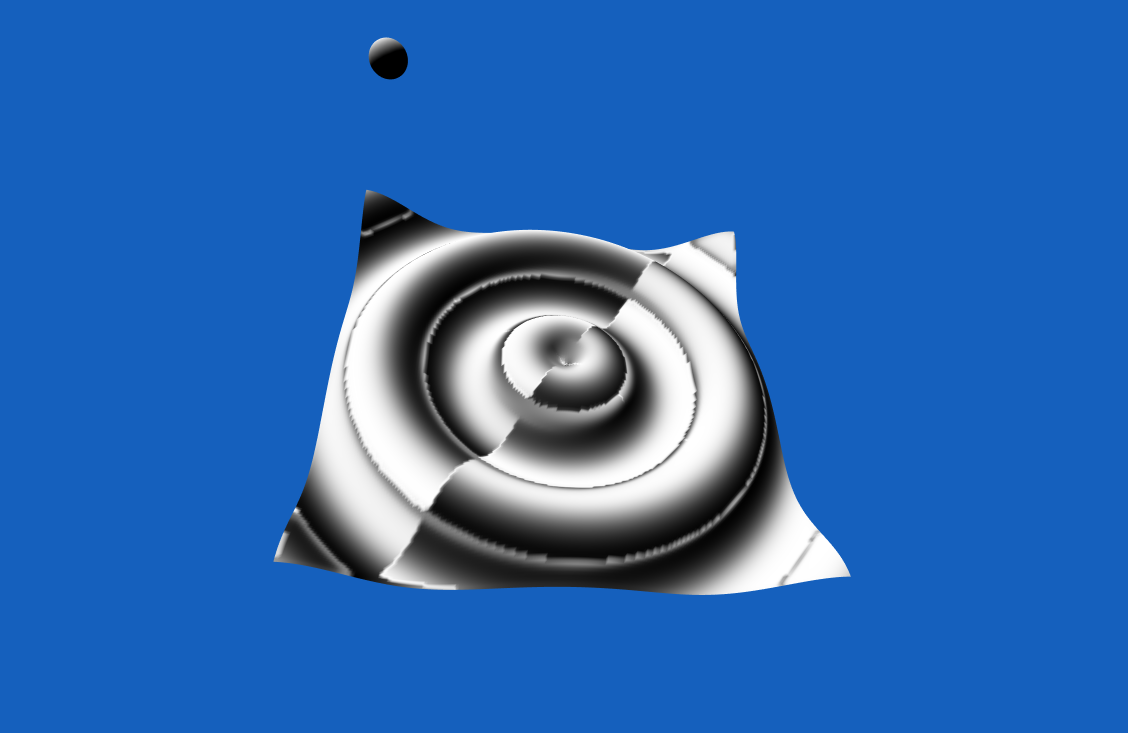
\includegraphics[scale=0.3]{Images/Essais/Essai_1_s_toy.png}
    \caption{"Essai 1 : Toy avec $S\theta$ "}
 \end{figure}



\begin{figure}[thb]
	\centering
    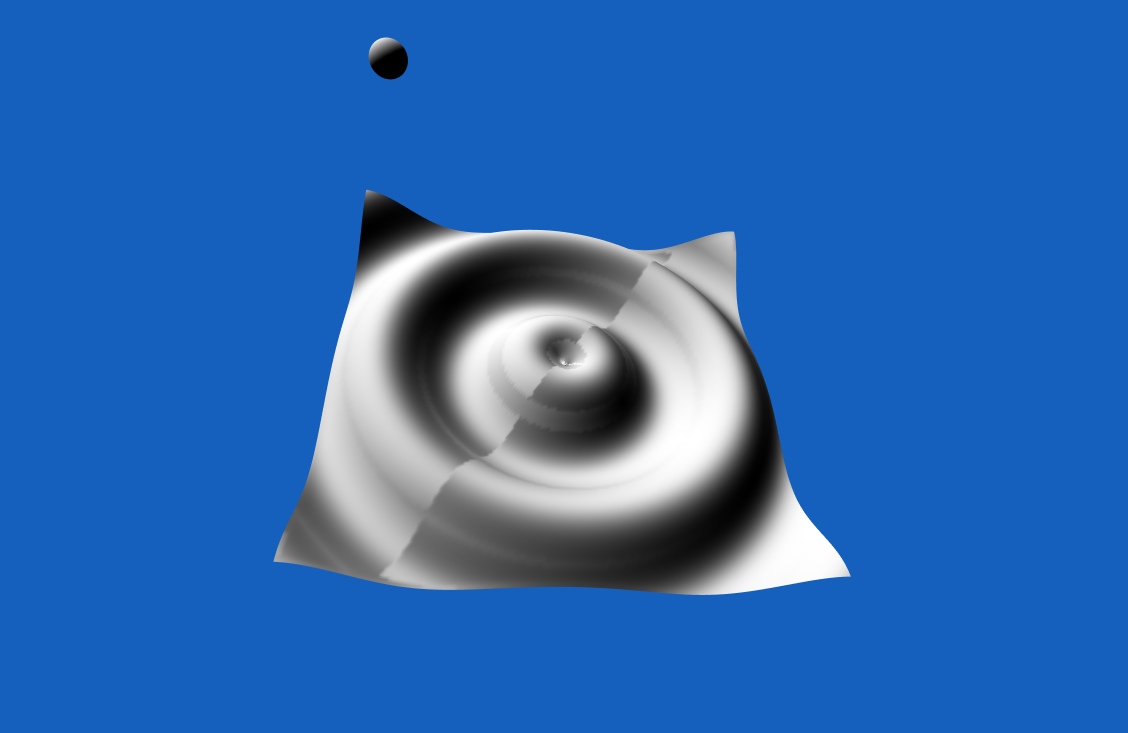
\includegraphics[scale=0.3]{Images/Essais/Essai_1_c_toy.png}
    \caption{"Essai 1 : Toy avec $C\theta$ "}
 \end{figure}


\begin{figure}[thb]
	\centering
    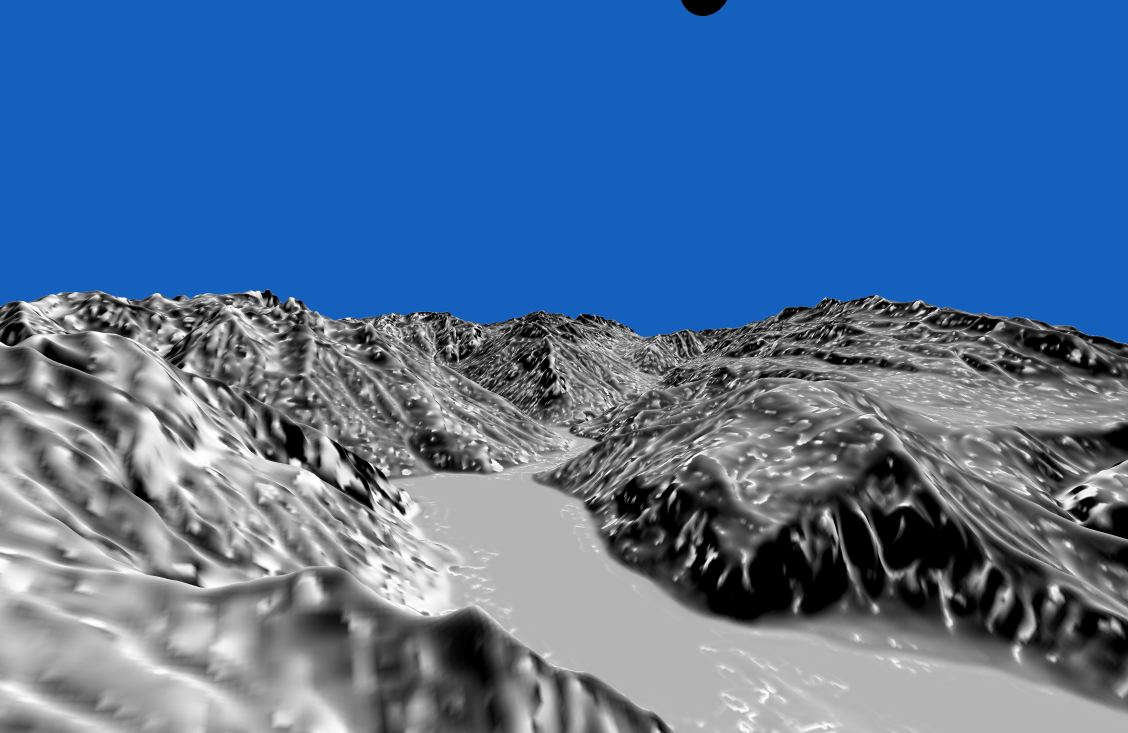
\includegraphics[scale=0.3]{Images/Essais/Essai_1_s_mount.png}
    \caption{"Essai 1 : Montagne avec $S\theta$ "}
 \end{figure}


\begin{figure}[thb]
	\centering
    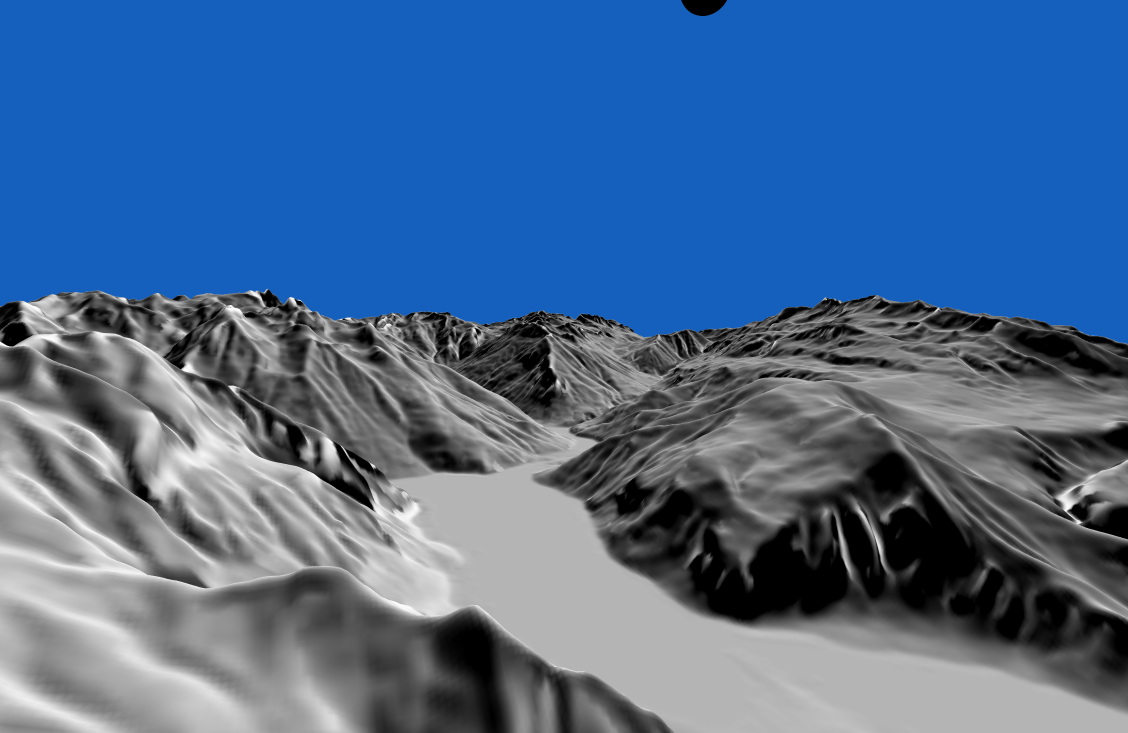
\includegraphics[scale=0.3]{Images/Essais/Essai_1_c_mount.png}
    \caption{"Essai 1 : Montagne avec $S\theta$ "}
 \end{figure}



\subsection{Essai 2}

\subsubsection{Principe}
Ici on prend le même principe que l'essaie 1 , mais on supprimer les facteurs $S$ et $C$ et on en créer un autre $F$ qui a pour butter de supprimer la discontinuité quand la lumière orthogonal.\\

Pour ce faire : On découpe $\theta$ avec $T$ une constante arbitraire dans l'intervale $[0,\frac{\pi}{2}]$



\[ \theta = 
\left\{
    \begin{array}{ll}
        \theta * F & \mbox{si } |\theta| > T \\
		\theta  & \mbox{sinon}				
    \end{array}
\right.
\]

Avec $F$ une interpolation d'Hermite de $|\theta| $ entre $T$ et $\frac{\pi}{2}$




\subsubsection{Résultats}



\begin{figure}[!h]
	\centering
    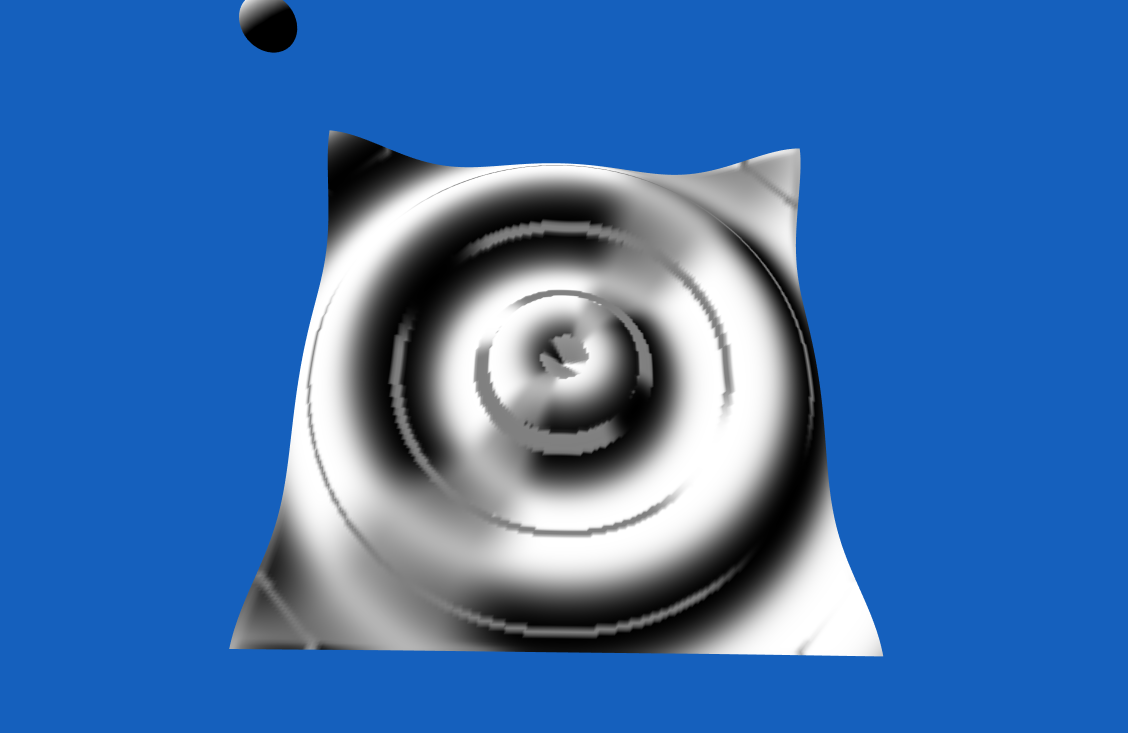
\includegraphics[scale=0.3]{Images/Essais/Essai_2_toy.png}
    \caption{"Essai 2 : Toy avec correction lumière"}
 \end{figure}


\subsection{Essai 3}

\subsubsection{Principe}
On continu sur la lancé de l'essai 2 et on essaye de corriger la 2eme discontinuité en prenant la curvature la plus aligné a la normals. Resultat : ça marche dans le cas du torus , mais pas dans le cas de la montagne ou avec le torus et le bruit de perlin. 

\subsubsection{Résultats}

\begin{figure}[thb]
	\centering
    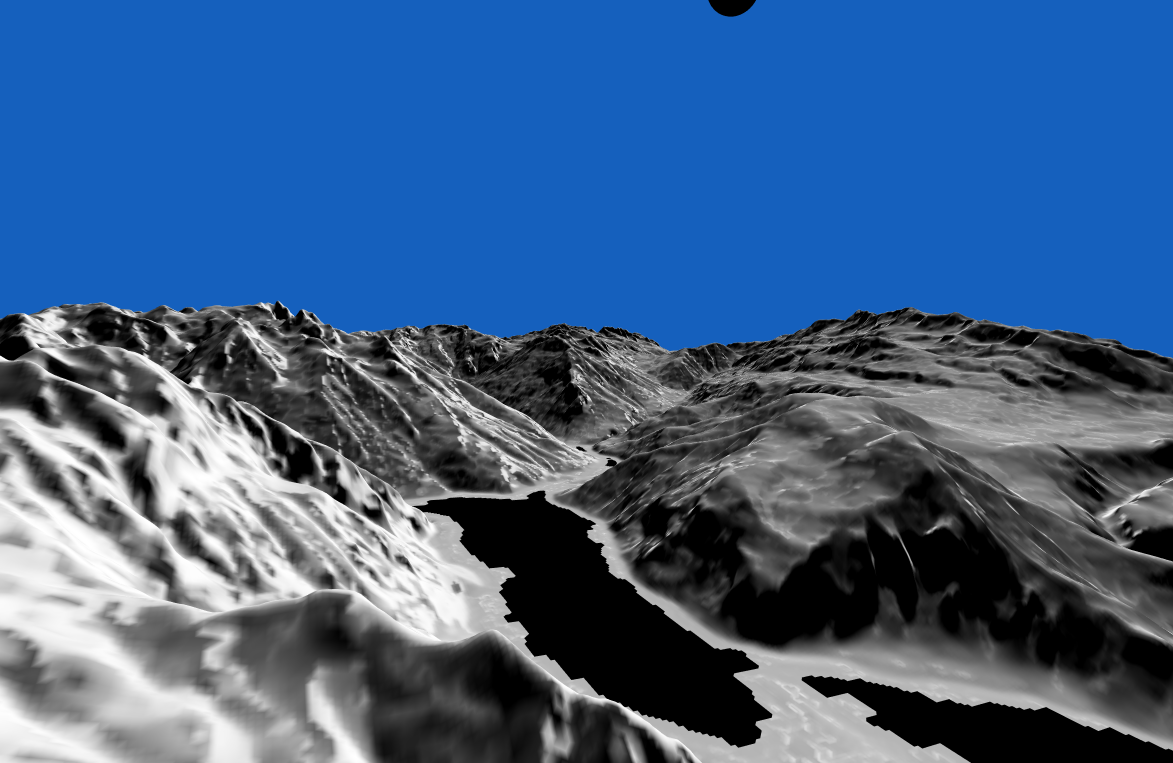
\includegraphics[scale=0.3]{Images/Essais/Essai_3_mount.png}
    \caption{"Essai 3 : Montagne correction Lumière+Normal"}
 \end{figure}

\begin{figure}[thb]
	\centering
    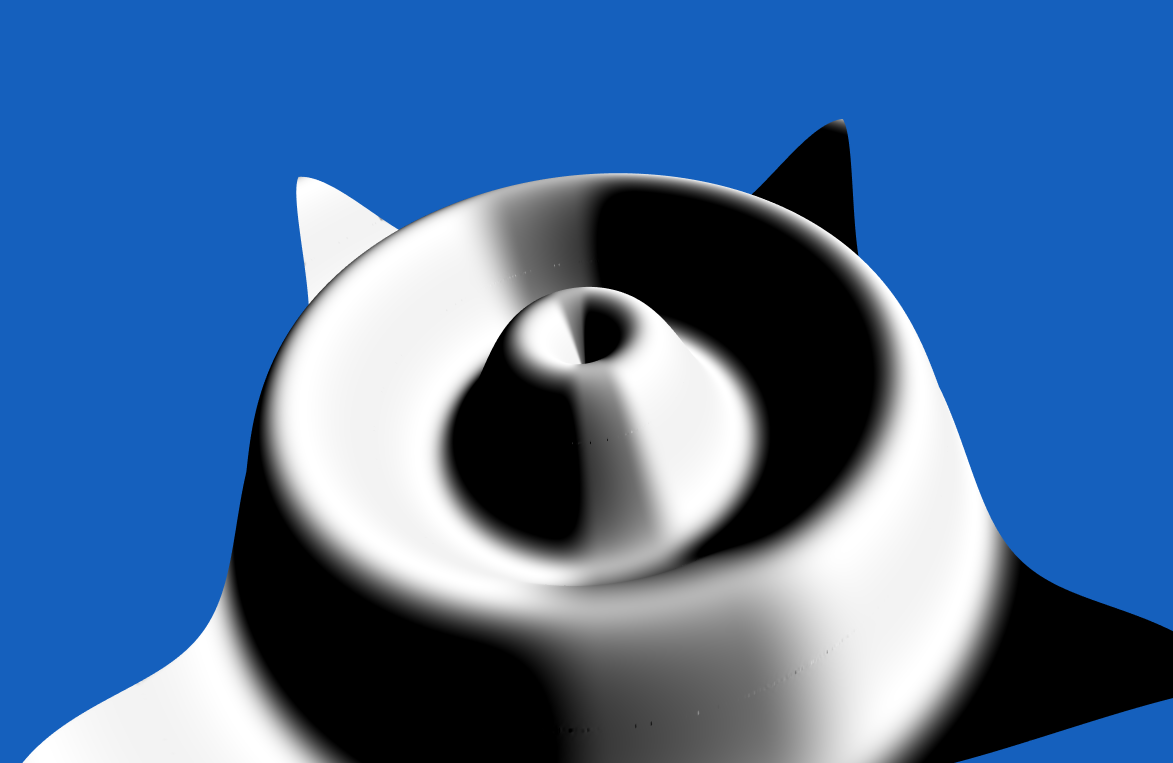
\includegraphics[scale=0.3]{Images/Essais/Essai_3_toy.png}
    \caption{"Essai 3 : Toy correction Lumière+Normal"}
 \end{figure}


\subsection{Essai 4}


\subsubsection{Principe}
On change le moyen de calculer la curvature. En effet , il y a trop d'information dans le resultat, ce qui provoque les discontinuité. Au final , on veut une unique information en chaque point, dans quel sens est ma pente. Donc une dérivé sur la carte de hauteur.
Ainsi on introduit un nouveau shader : slint. Qui permet de calculer cette dérivé . Ensuite on calcule la lumière avec cette dérivé de la même manière qu'avec la curvature (cf Essai 2). 
Ca corrige beaucoup de probleme mais il y en reste 2: 
\begin{itemize}
\item Quand la dérivé est nul, il y a une petite discontinuité.
\item Il y a un problème de résolution. La lumière est pixélisé ce qui est pas très jolie.
\end{itemize}
Est-ce qu'un léger flou sur l'intensité de la lumière réglerait ces 2 problèmes ? Y'a t'il d'autre solution possible ?

\subsubsection{Résultats}


\begin{figure}[thb]
	\centering
    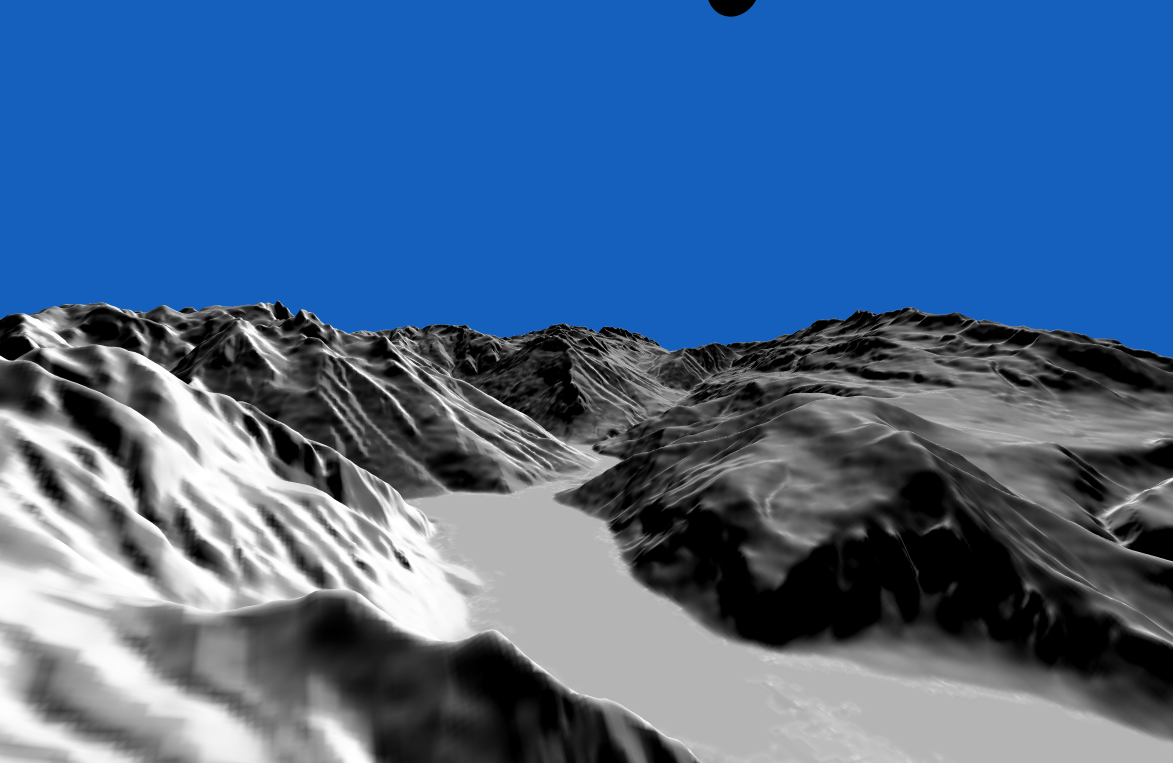
\includegraphics[scale=0.3]{Images/Essais/Essai_4_mount.png}
    \caption{"Essai 4 : montagne"}
 \end{figure}



\begin{figure}[thb]
	\centering
    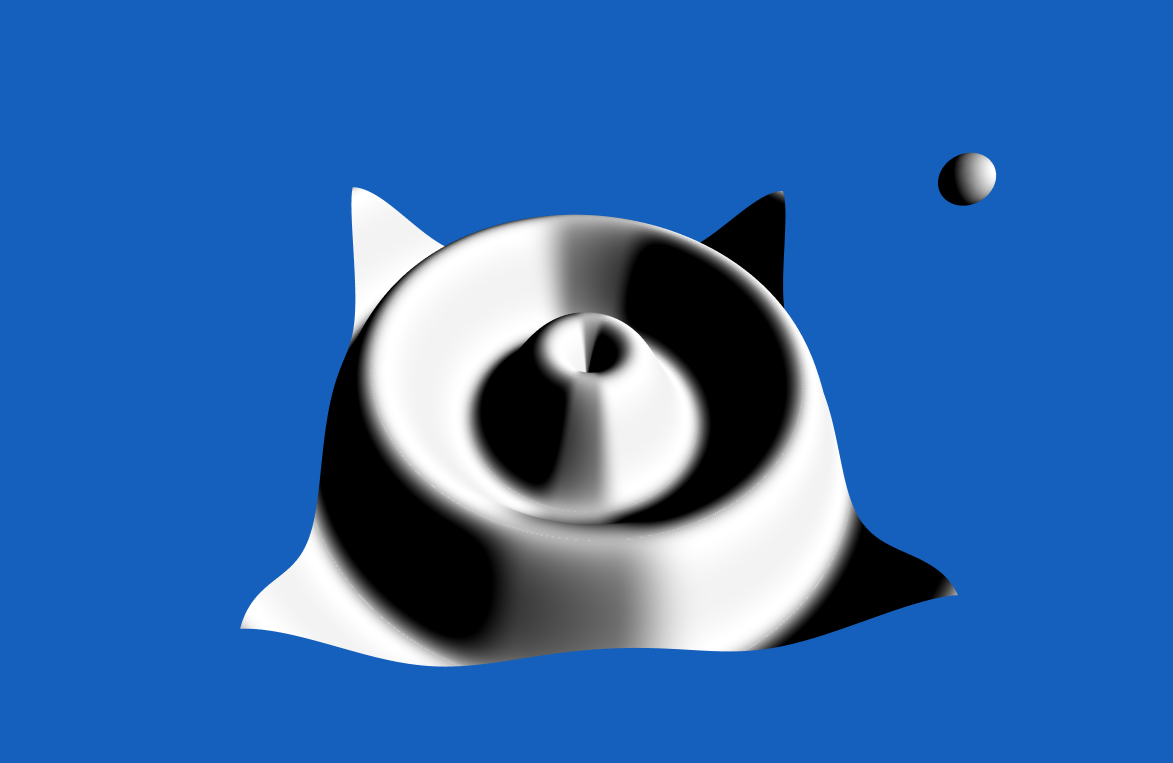
\includegraphics[scale=0.3]{Images/Essais/Essai_4_toy.png}
    \caption{"Essai 4 : Toy "}
 \end{figure}

\begin{figure}[thb]
	\centering
    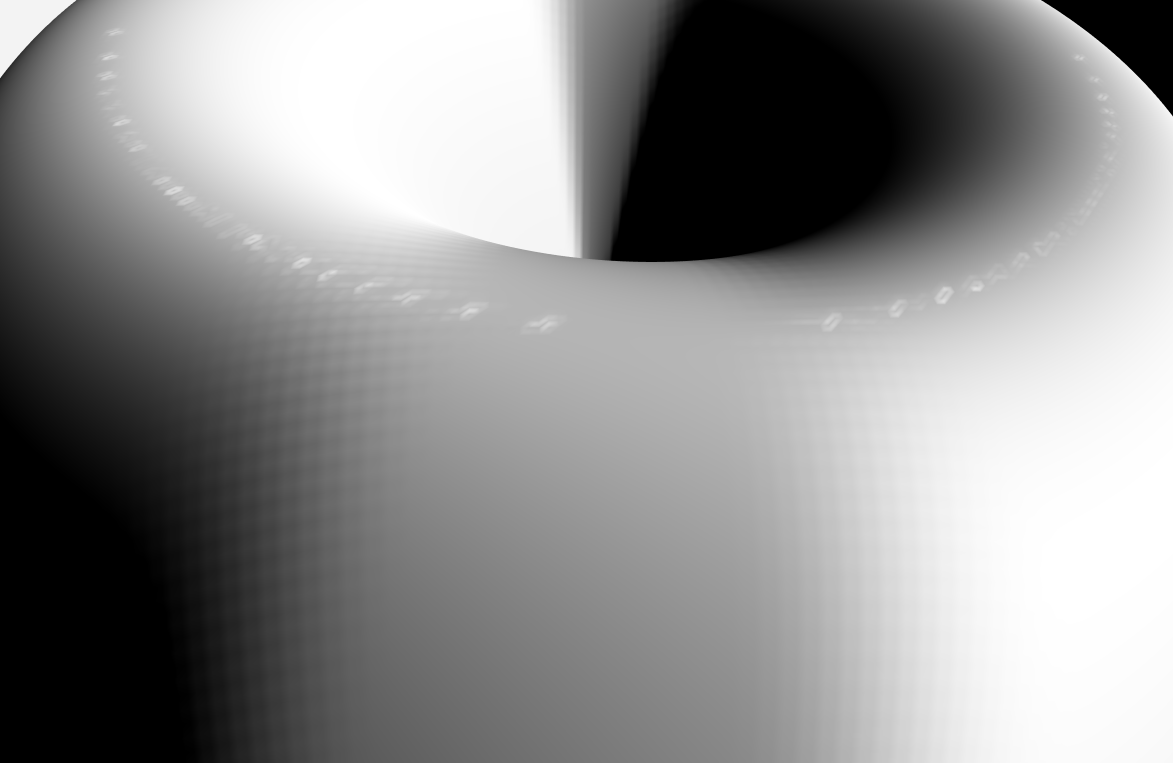
\includegraphics[scale=0.3]{Images/Essais/Essai_4_toy_zoom.png}
    \caption{"Essai 4 : Toy  - zoom"}
 \end{figure}
 
\subsection{Essai 5}
\subsubsection{Principe}
Pour le problème des discontinuités , le problème venait de l'implémentation de la dérivé partiel par GLSL. En effet , il va uniquement faire la différence entre le pixel courant et le pixel courant +1 en x et en y (Plus d'info ici : \url{http://www.aclockworkberry.com/shader-derivative-functions/} ) Donc en réimplantant la fonction mais en prenant en compte des pixel en -1 et +1 en x et y , on réduit drastiquement les discontinuité et on obtient un résultat plus convaincant. Mais il y en a toujours quand la dérivée est nul. 


\[dx_i = \frac{x_i - x_{i-1} + x_{i+1} - x_{i} }{2}\]

\[dy_i = \frac{y_i - y_{i-1} + y_{i+1} - y_{i} }{2}\]


Par contre , on observe que quand on augmente le flou gaussien , la pixelisation de la lumière diminue. 

\subsubsection{Résultats}
\begin{figure}[thb]
	\centering
    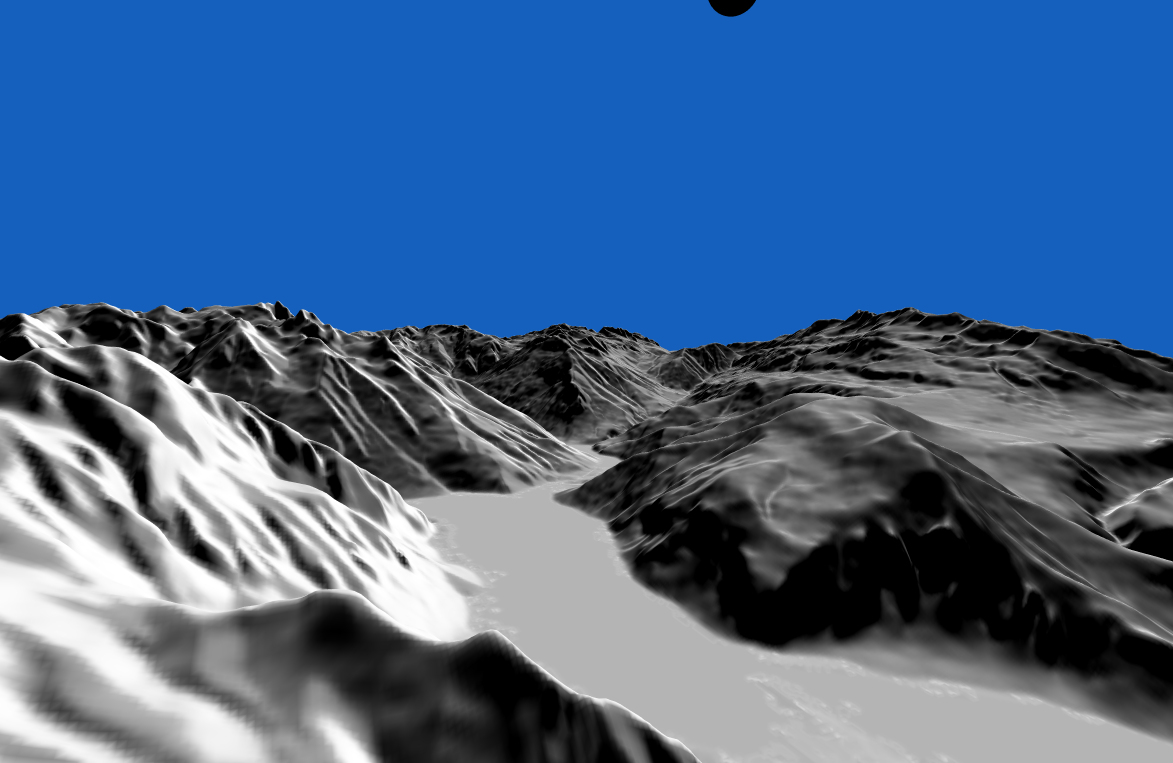
\includegraphics[scale=0.3]{Images/Essais/Essai_5_mount.png}
    \caption{"Essai 5 : montagne"}
 \end{figure}



\begin{figure}[thb]
	\centering
    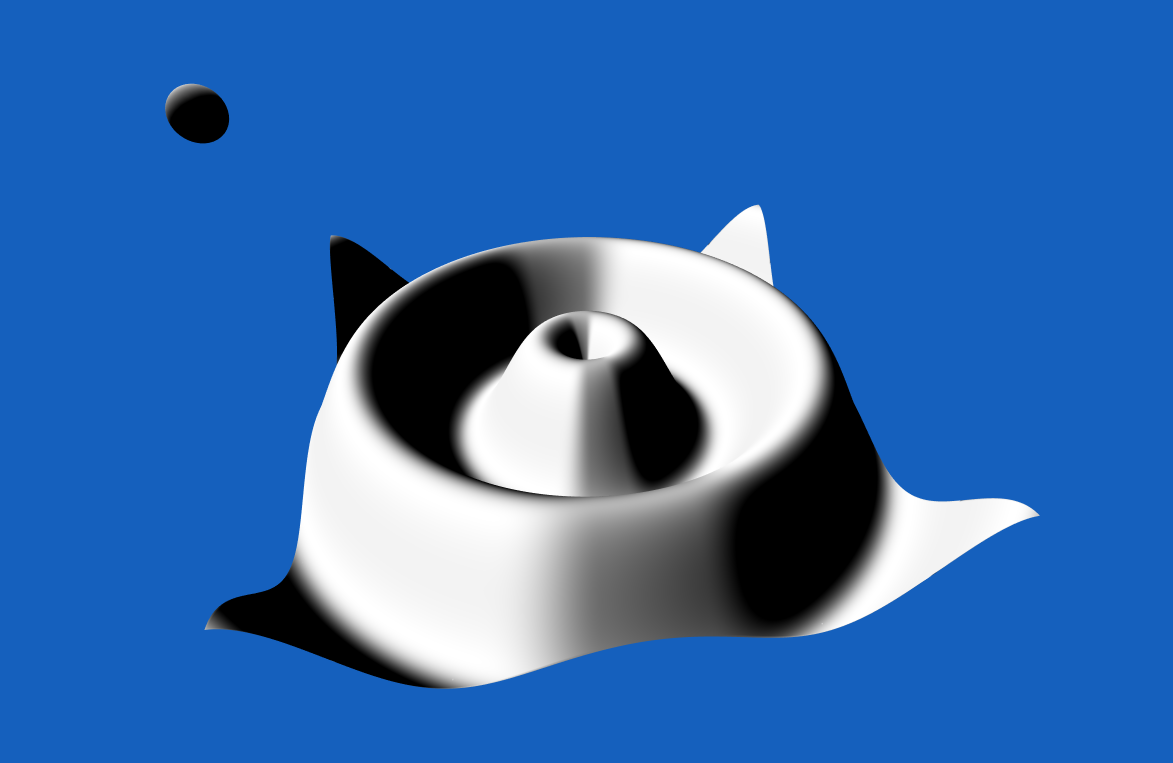
\includegraphics[scale=0.3]{Images/Essais/Essai_5_toy.png}
    \caption{"Essai 5 : Toy "}
 \end{figure}

\begin{figure}[thb]
	\centering
    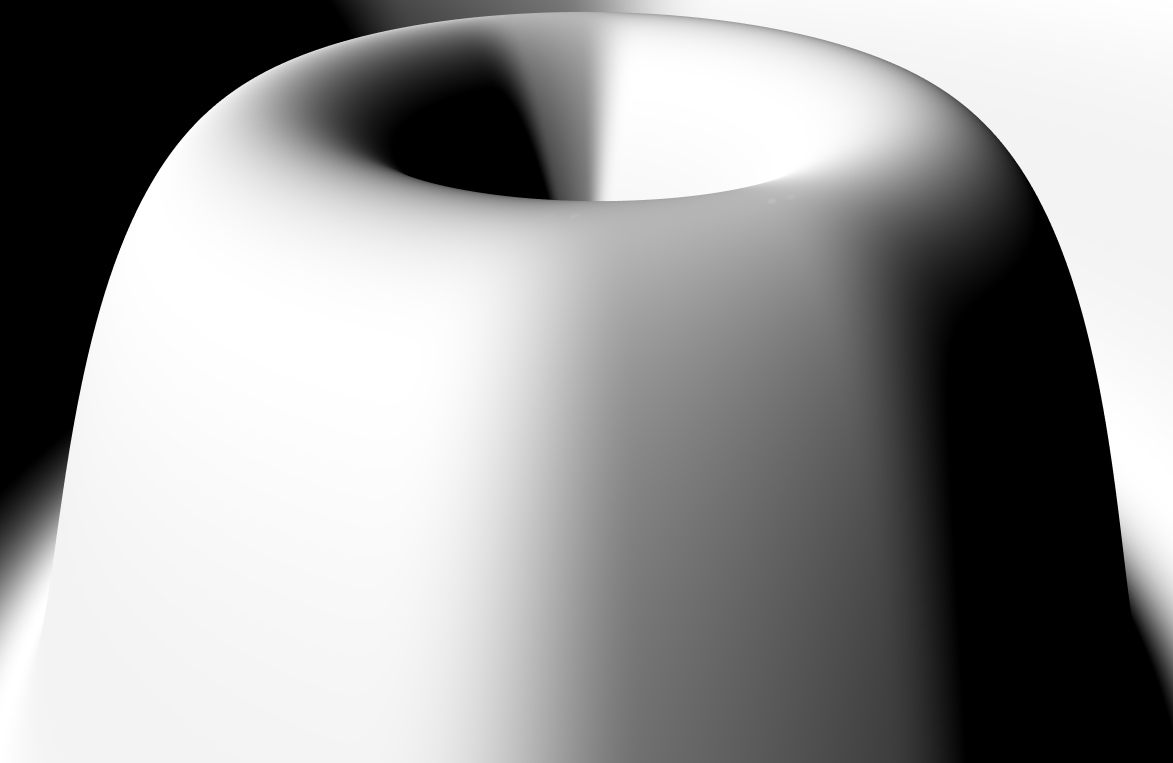
\includegraphics[scale=0.3]{Images/Essais/Essai_5_toy_zoom.png}
    \caption{"Essai 5 : Toy  - zoom"}
 \end{figure}
 
 \subsection{Essai 6}
\subsubsection{Principe}
On continu sur l'essai 5 et on supprime la dernière discontinuité : 
Le problème vient de la transition entre le moment où on a une direction de pente et le moment où la direction est nul. Pour ce faire on fait 2 chose. D'abord on modifie la manière de récupérer la direction de la pente. Au lieu de recalculer la dérivé , on prend celle déjà calculé : les normals. Ici on prend que les valeurs x,y des normals.
Ensuite pour supprimer la discontinuité , on multiplie l'angle de modification par la taille de $\vec{(n_x,n_y)}$.
Et voila , on a enfin un déformation de la lumière propre sans discontinuité et qui fait ce qu'on veut (c'est à dire s'aligner avec la pente). 
\subsubsection{Résultats}
\begin{figure}[thb]
	\centering
    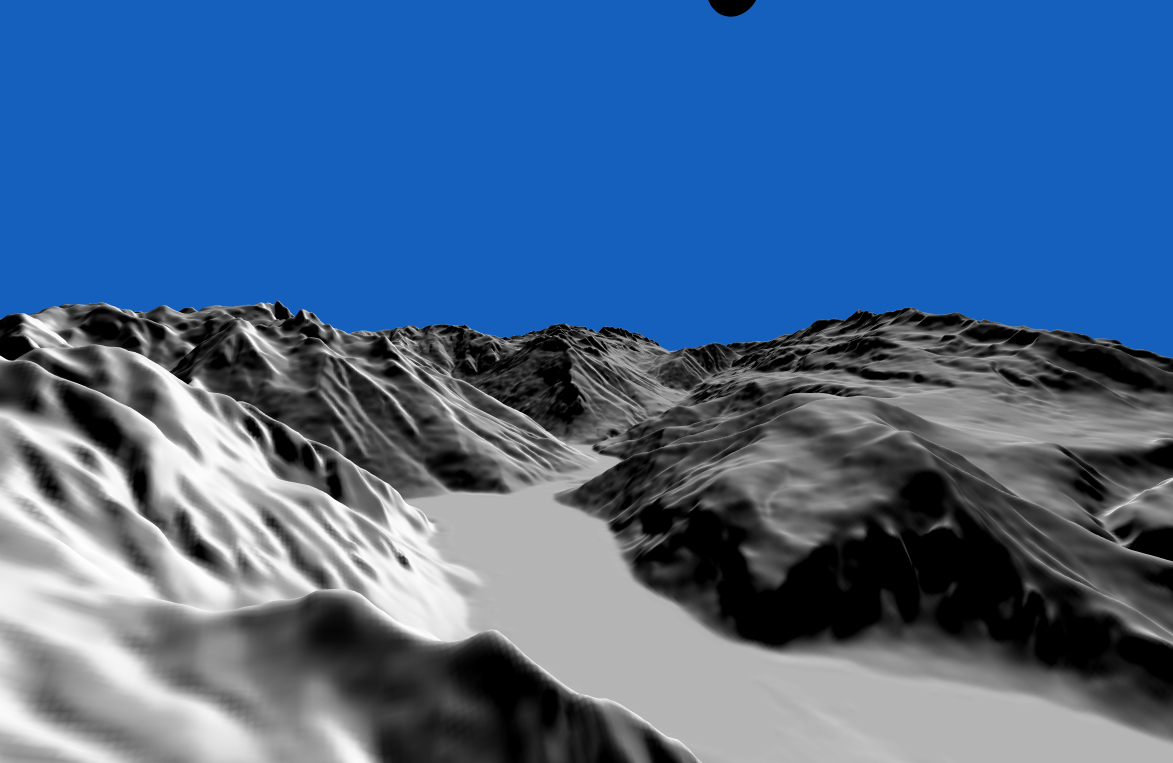
\includegraphics[scale=0.3]{Images/Essais/Essai_6_mount.png}
    \caption{"Essai 6 : montagne"}
 \end{figure}



\begin{figure}[thb]
	\centering
    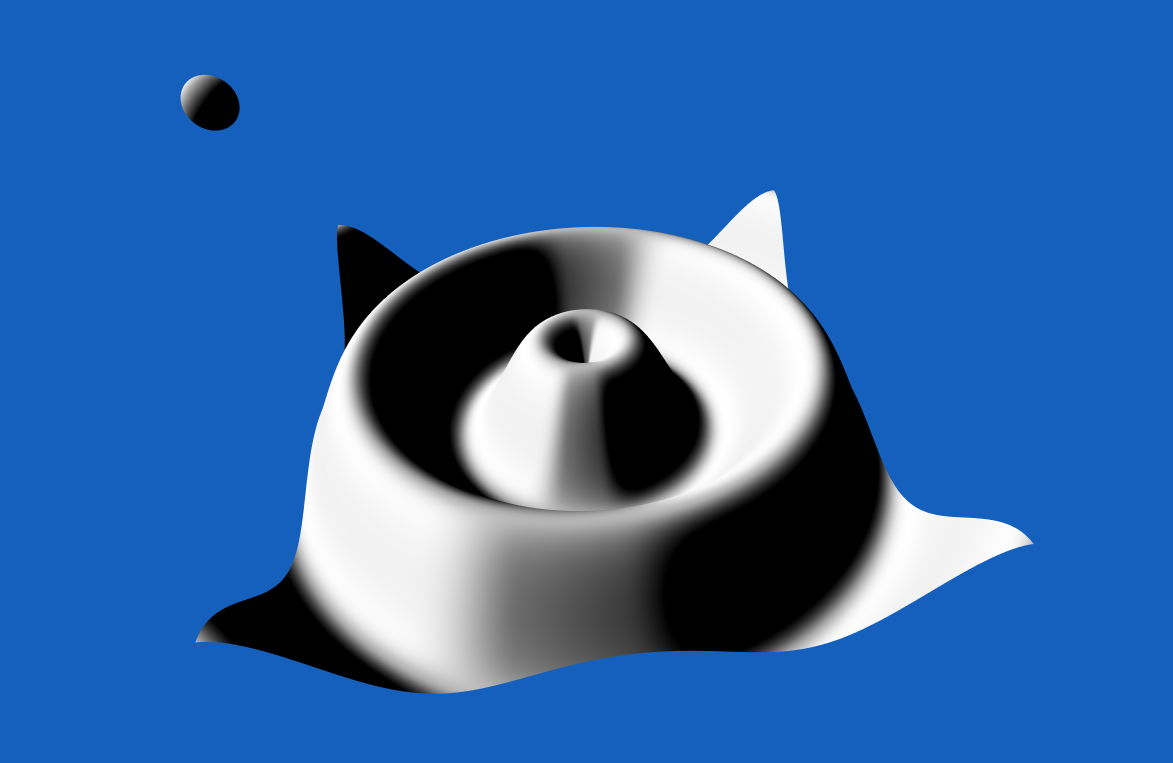
\includegraphics[scale=0.3]{Images/Essais/Essai_6_toy.png}
    \caption{"Essai 5 : Toy "}
 \end{figure}

\begin{figure}[thb]
	\centering
    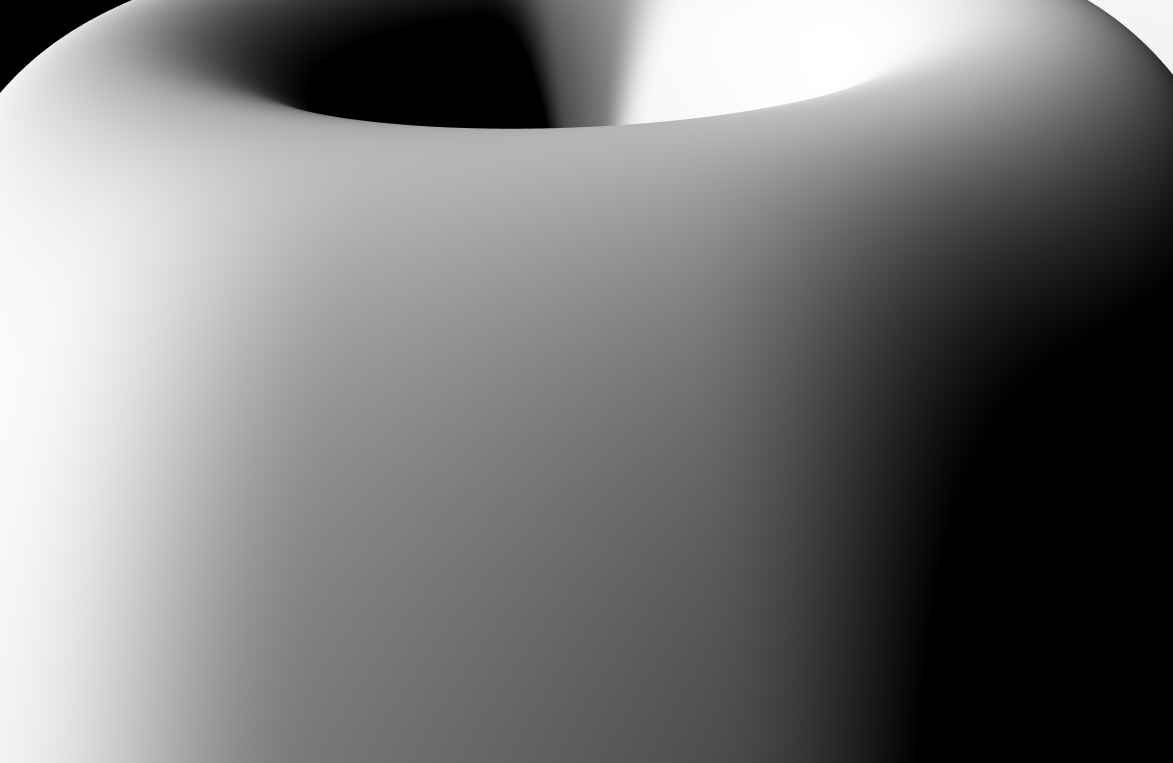
\includegraphics[scale=0.3]{Images/Essais/Essai_6_toy_zoom.png}
    \caption{"Essai 5 : Toy  - zoom"}
 \end{figure}
 
 
 %%%% VOIR OVERLEAF : https://www.overleaf.com/15938415jvbnzcxbnxhm
\section{Questions}

Questions principales :
\begin{itemize}
\item Qu'est-ce qu'on veut voir ?
\item Qu'est-ce qu'est une feature ? Comment la définir ? Comment la détecter ? 
\item Quel features on souhaite voir ? Seulement les verticales ? Seulement les horizontales ? Les deux ? Est-ce qu'il n'y a pas uniquement des features verticales ? 
\item Comment les mettre en valeurs ? Mettre la lumière perpendiculaire ?
\item Qu'est que ça veut dire, mettre la lumière perpendiculaire ? A quoi ? 
\item Qu'est-ce que notre approche apporte par rapport à un ombrage classique ? 
\item Est-ce que on reste fidèle au style de Novat ?
\item Est-ce qu'une cohérence global est importante ? 
\item Est-ce qu'une cohérence local est importante ? 
\item Faire le flou d'un Novat, est-ce que il y des choses intéressante qui ressorte ? 
\item Comment valider une méthode ? 
\item Comment valider une partie de méthode ? 
\item Dans les partie ombragé des montagnes , y'a t'il des ombres porté ou est-ce seulement des variations d'ombrage ? 
\end{itemize}

Les leviers qu'on a : 

\begin{itemize}
\item Orientation de la lumière.
\item Méthode d'ombrage et d'ombre porté.
\item Flou gaussien.
\item Multi-Échelle. 
\end{itemize}

Les questions qui correspondent :

\begin{itemize}
\item Quel méthode d'ombrage utiliser ? phong ( $max(l\cdot d, 0)$ ) , $ l\cdot d*0.5 + 0.5$ , cel shading ?
\item Quel méthode d'ombre portée utiliser ? 
\item Comment modifier l'orientation de notre lumière ? En fonction de la pente ? De la courbure ?
\item Est-ce qu'il faut aligner totalement la lumière avec la pente ? Est-ce que décaler un peu par rapport à la pente à du sens ? Si oui , de combien il faut décaler ? 
  
\item Est-ce qu'il faut empêcher la lumière local d'être à moins de 90 par rapport à la lumière original ? 
\item Modifier uniquement l'azimut ? Modifier aussi l'élévation ? 
\item Faut il garder la même orientation de lumière pour calculer l'ombrage et les ombres portés ?
\item Si non , quel différence on veut avoir entre l'ombrage et les ombres portés ?
\item Faut-il empêcher le retournement de la lumière , Si non , faut-il faire une différence entre la lumière aligné et non aligné avec la lumière global ? 
\item Le flou gaussien est-il une bonne idée pour faire du multi echelle ? Est-ce qu'il existe d'autre solution adapté à notre situation ? 
\item Faut-il utiliser un flou sur la carte de hauteur pour avoir uniquement les grosses montagnes lissé ?
\item Si oui , calcule de la lumière uniquement sur le flou ? Sur le normal et le flou ? Sur plusieurs flou ? 
\item Si plusieurs flou, comment les combiner ? 

\end{itemize} 



\subsection{Mes réponses}
Question principales :

\textit{}
Novat avec ses ombres indique plus des modification de terrain que de la lumière.
\textit{Qu'est-ce qu'est une feature ? Comment la définir ? Comment la détecter ? }\\
Ca nous sert à voir la forme de la montagne a plus ou moins grande échelle. Quand c'est plat, faut voir que c'est plat. Pas rajouter de la forme. Sans rajouter , ni cacher.  
Définition d'une feature : C'est l'opposé de plat. C'est une zone dont les normales ne sont pas constante dans au moins une direction. La direction où les normales sont constante est la direction de la feature. \\
\textit{Quel features on souhaite voir ? Seulement les verticales ? Seulement les horizontales ? Les deux ? Est-ce qu'il n'y a pas uniquement des features verticales ?}\\ 
Dans l'idéal on souhaiterai voir toutes les features vertical et horizontal. De plus il n'y a pas que des features vertical , les horizontales existe aussi et elle sont tout aussi importante car c'est généralement des barres rocheuses. \\
Pour donner a voir une bosse , c'est avoir un coté blanc , un coté noir et différent de la surface où c'est posé. \\
\textit{Comment les mettre en valeurs ? Mettre la lumière perpendiculaire ?}\\
Le meilleur moyen de mettre en valeur une feature c'est d'avoir une lumière perpendiculaire à sa direction principal. \\
Les verticales c'est mis en valeur par l'ombrage et les horizontales c'est mis en valeur par les ombres portées. \\
\textit{Qu'est que ça veut dire, mettre la lumière perpendiculaire ? A quoi ? }\\
Ce qui décrit le mieux un feature c'est la courbure, Seulement la courbure max a pour soucis majeur de ne pas être toujours dans le sens de la pente. Il peut qu'elle soit dans un autre sens. Hors si on veut que la direction soit globalement celui de la pente, autant prendre directement la pente.  \\  
La pente c'est la dérivé 1er de la carte de hauteur (normal) la courbure c'est la dérivé seconde de la carte de hauteur (soit la dérivé des normals). \\
\textit{Qu'est-ce que notre approche apporte par rapport à un ombrage classique ? }\\
On souhaite mieux mettre en valeur les features en alignant la lumière avec ces features.  \\
\textit{Est-ce que on reste fidèle au style de Novat ?}\\
Difficile à dire.\\
Le but est laisser à voir les même choses que lui.
\textit{Est-ce qu'une cohérence global est importante ? }\\
 Non une cohérence global n'est pas importante car elle n'est pas présente dans les œuvres de Novat et ça ne gène pas l'oeil du lecteur. \\
 Recherche papier sur la perception des ombres et la cohérence des ombres. \\
\textit{Est-ce qu'une cohérence local est importante ? }\\
Oui car sinon on peut se retrouver avec des discontinuités non voulue qui casse la lecture.\\
\textit{Faire le flou d'un Novat, est-ce que il y des choses intéressante qui ressorte ? }\\
TODO \\
\textit{Comment valider une méthode ? }\\
Faire des exemples jouet avec des features dessus et vérifié que le résultat obtenu est bien ce lui qu'on veut. Faire une comparaison numérique entre notre méthode et la méthode classique la plus proche. Montrer le résultat à des experts (Novat) . Montrer le résultat à un ensemble d'utilisateurs lambda. \\
\textit{Comment valider une partie de méthode ? }\\
?\\
\textit{Dans les partie ombragé des montagnes , y'a t'il des ombres porté ou est-ce seulement des variations d'ombrage ? }\\
Difficile à dire , mais je dirais que non. Il y a uniquement l'ombre des arbres qui peuvent se rajouter. Pas celui d'autres bosses. \\ 





Question levier : 



\textit{ Quel méthode d'ombrage utiliser ? phong ( $max(l\cdot d, 0)$ ) , $ l\cdot d*0.5 + 0.5$ , cel shading ?}\\
A Tester mais la 2eme methode pourrai etre meilleur car ça ne cacherai pas toute les partie dans l'ombre. \\
\textit{ Quel méthode d'ombre portée utiliser ? }\\
 Il faudrait une méthode qui permette d'avoir des ombres porté plus anguleuse et avec un dégradé entre le centre d'une ombre et le bord . \\
 Morphologie mathématique (traitement d'image). 
\textit{ Comment modifier l'orientation de notre lumière ? En fonction de la pente ? De la courbure ?}\\
Si on oriente la lumière en fonction de la pente , on se retrouve avec les discontinuité décrite plus haut. Orienter par rapport à la pente semble satisfaisant et suffisant.\\
\textit{ Est-ce qu'il faut aligner totalement la lumière avec la pente ? Est-ce que décaler un peu par rapport à la pente à du sens ? Si oui , de combien il faut décaler ? }\\
A tester. \\
  
\textit{ Est-ce qu'il faut empêcher la lumière local d'être à moins de 90 par rapport à la lumière original ? }\\
Il faut définir ce qu'on veut voir dans les parties dans l'ombre. Dans ces partie on souhaiterai voir quelque chose. Pas avoir un noir totale. Hors, c'est seulement le cas dans les grosses montagnes : En effet dans le cas d'une montagne , on a un versant à l'ombre , l'autre au soleil. Sur le versant au soleil , pas de problème. Sur le versant à l'ombre , on voudrait voir quel que chose. Donc on pourrait retourner la lumière. Seulement , il faut faire attention. Déjà il faut quand même garder cette aspect ombre/lumière (aspect qui peut être fait par les ombres portées). Ensuite , il faudrait avoir cette possibilité d'inversion uniquement a grande échelle. Il ne faudrait pas que les petites bosses soit toutes blanches et donc totalement effacé. \\
\textit{ Modifier uniquement l'azimut ? Modifier aussi l'élévation ? }\\
Pour l'ombrage , la hauteur de la lumière peut être libre à l'utilisateur. Mais pour les ombres portées c'est différent. Je pense que ce qui est important c'est la taille des ombres portée que l'utilisateur doit sélectionner mais pas la hauteur directement. En effet, sur un haute montagne on veut que l'ombre s'arrête à un endroit proche de ses pieds. Mais pour une petite bosse , on veut que l'ombre soit bien plus important proportionnellement : on veut avoir une lumière bien plus rasante par rapport à la bosse. C'est assez complexe au final. 
Ça va dépendre de la différence entre l'angle de la pente (dans une echelle plus large) par rapport à l'angle (pitch) de la lumière. \\
\textit{ Faut il garder la même orientation de lumière pour calculer l'ombrage et les ombres portés ?}\\
Il faudrait les séparer dans un premier temps, afin d'être plus libre et si au final , le calcule est le même alors on les fusionne.
\textit{ Si non , quel différence on veut avoir entre l'ombrage et les ombres portés ?}\\
Comme dit plus haut , l'azimute serai le même mais la hauteur changerai. 
\textit{ Faut-il empêcher le retournement de la lumière , Si non , faut-il faire une différence entre la lumière aligné et non aligné avec la lumière global (dans le même sens? }\\
je pense que c'est un soucis qui peut se régler avec la 2eme méthode d'ombrage. 
\textit{ Le flou gaussien est-il une bonne idée pour faire du multi echelle ? Est-ce qu'il existe d'autre solution adapté à notre situation ? }\\
C'est la seul méthode que je connaisse , s'il en existe d'autre je suis preneur. 
\textit{ Faut-il utiliser un flou sur la carte de hauteur pour avoir uniquement les grosses montagnes lissé ?}\\
Oui. Il faudrait un outils d'analyse pour détecter les échelles pertinente. 
\textit{ Si oui , calcule de la lumière uniquement sur le flou ? Sur le normal et le flou ? Sur plusieurs flou ? }\\
Plusieurs flou.
\textit{ Si plusieurs flou, comment les combiner ? }\\
Chaque flou prend en entrée une carte de lumière générée par un flou plus grande échelle.



\subsection{Ensemble des choses à tester}
\begin{itemize}
\item Pourquoi il se passe rien quand j'enlève l'inversion ? (BUG ?)
\item Le model  $max(l\cdot d, 0)$
\item Le model  $ l\cdot d*0.5 + 0.5$
\item Faire des model jouet plus complet : exemple sinusoide avec une bosse, puis un U. 




\end{itemize}


\section{Essai 7}
\subsection{Principe}
On change le model : on a donc 2 model : $max(l\cdot d, 0)$ (1) et  $max(l\cdot d, 0)$ (2) 
Et on fait des essais avec 4 direction de lumière (nord , sud, est , ouest). Et avec notre méthode et la méthode classique. 

\subsection{Resultats}
A gauche , on a le shading classsique , a gauche notre méthode. 
Model 1 :  $max(l\cdot d, 0)$ , model 2 :  $max(l\cdot d, 0)$.

\subsubsection{Nord , model 1}
\begin{tabular}{cc}
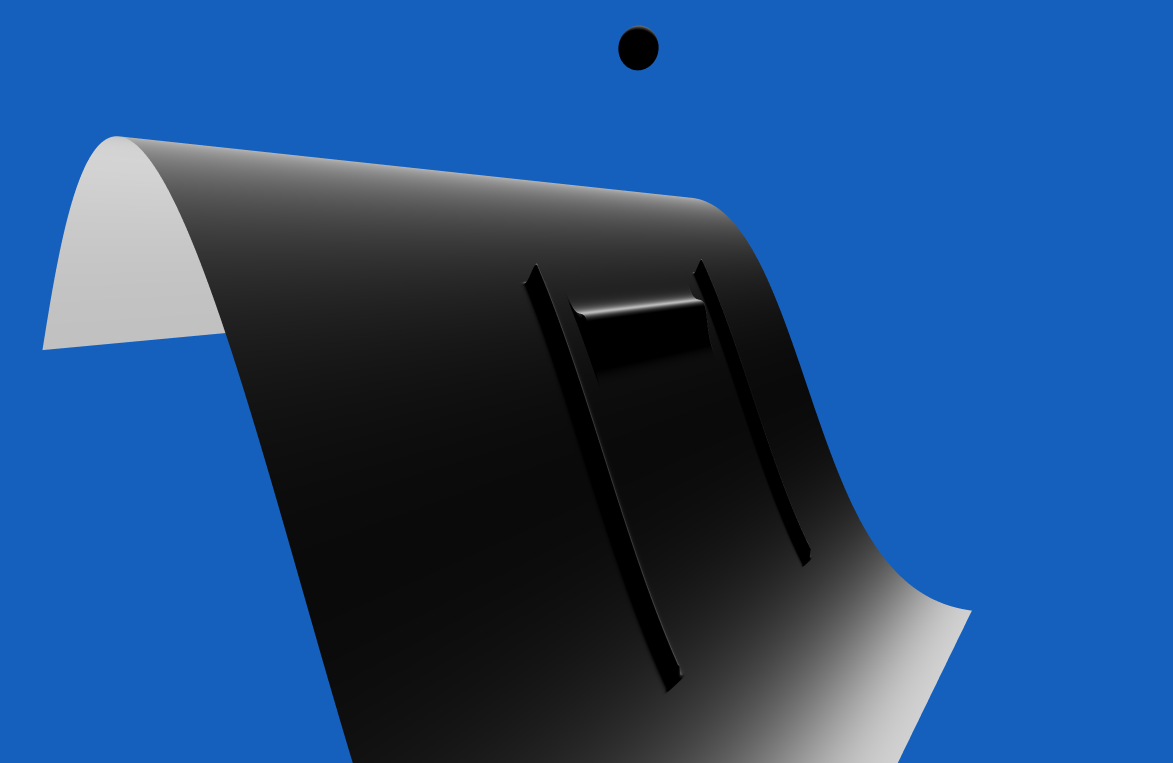
\includegraphics[width=0.4\textwidth]{Images/Essais/Essai_7_phong_North_0.png}
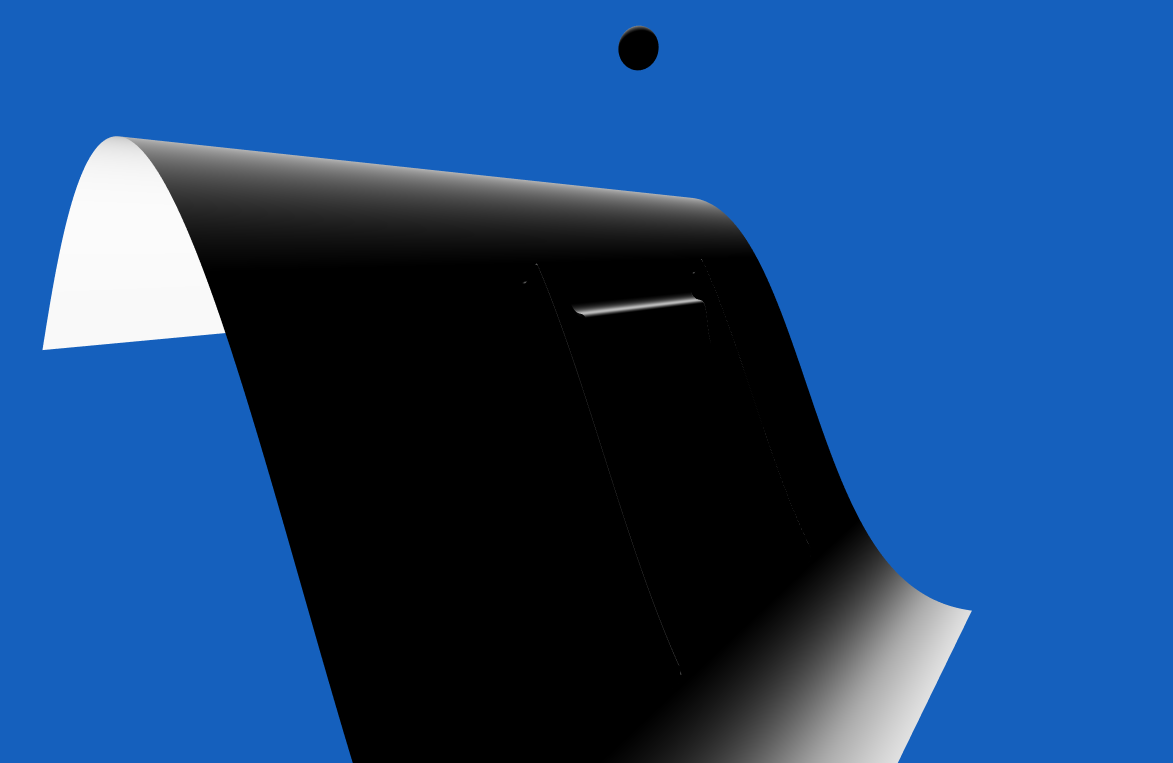
\includegraphics[width=0.4\textwidth]{Images/Essais/Essai_7_slint_North_0.png}
\end{tabular}

\subsubsection{Nord, model 2}
\begin{tabular}{cc}
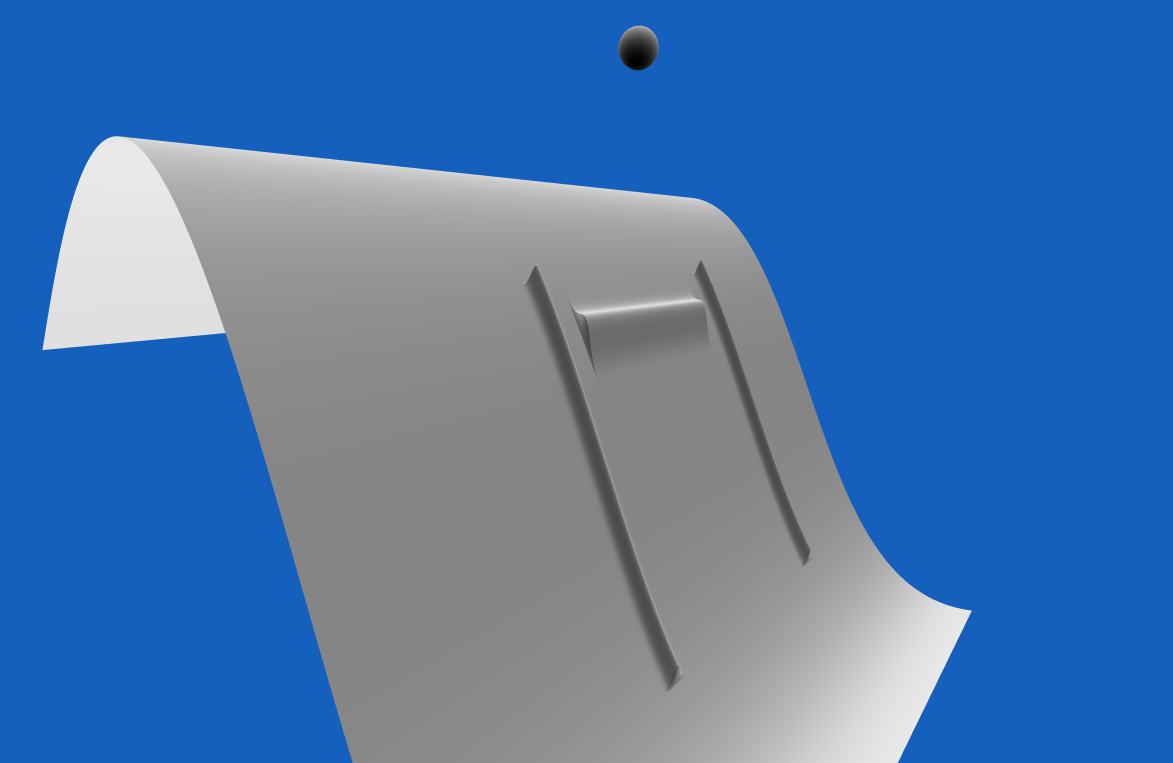
\includegraphics[width=0.4\textwidth]{Images/Essais/Essai_7_phong_North_1.png}
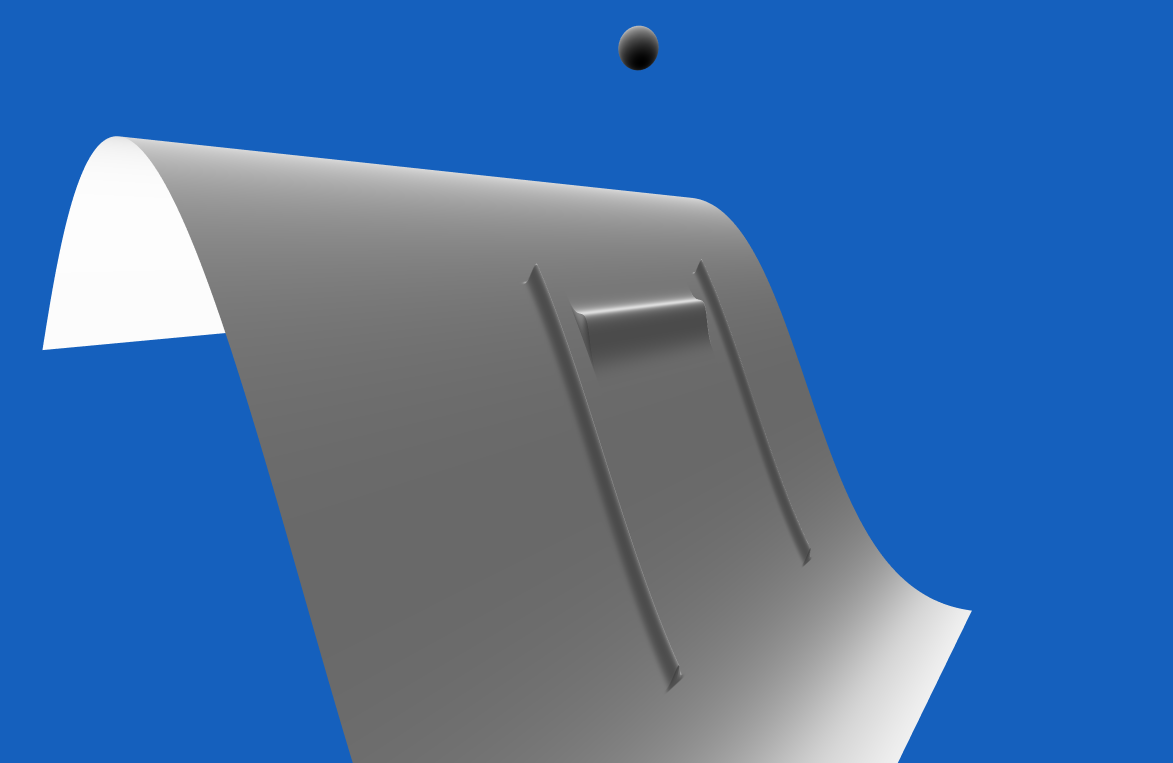
\includegraphics[width=0.4\textwidth]{Images/Essais/Essai_7_slint_North_1.png}
\end{tabular}
\subsubsection{Est, model 1}
\begin{tabular}{cc}
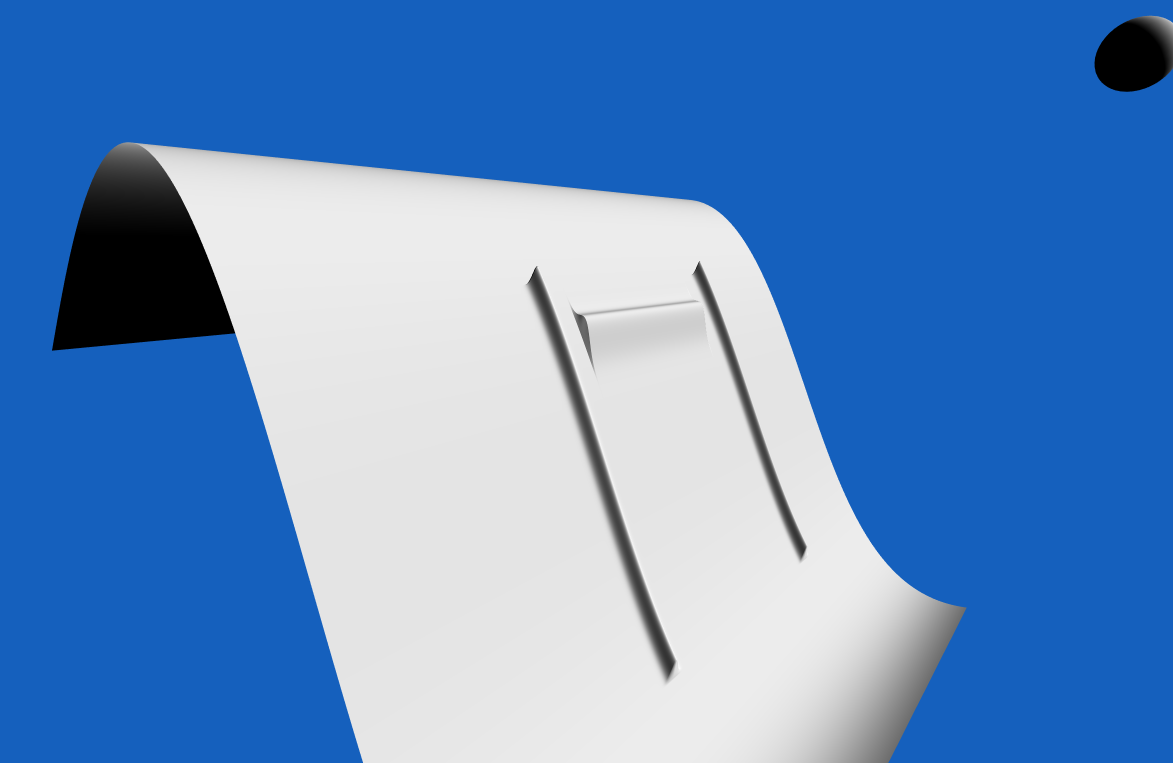
\includegraphics[width=0.4\textwidth]{Images/Essais/Essai_7_phong_East_0.png}
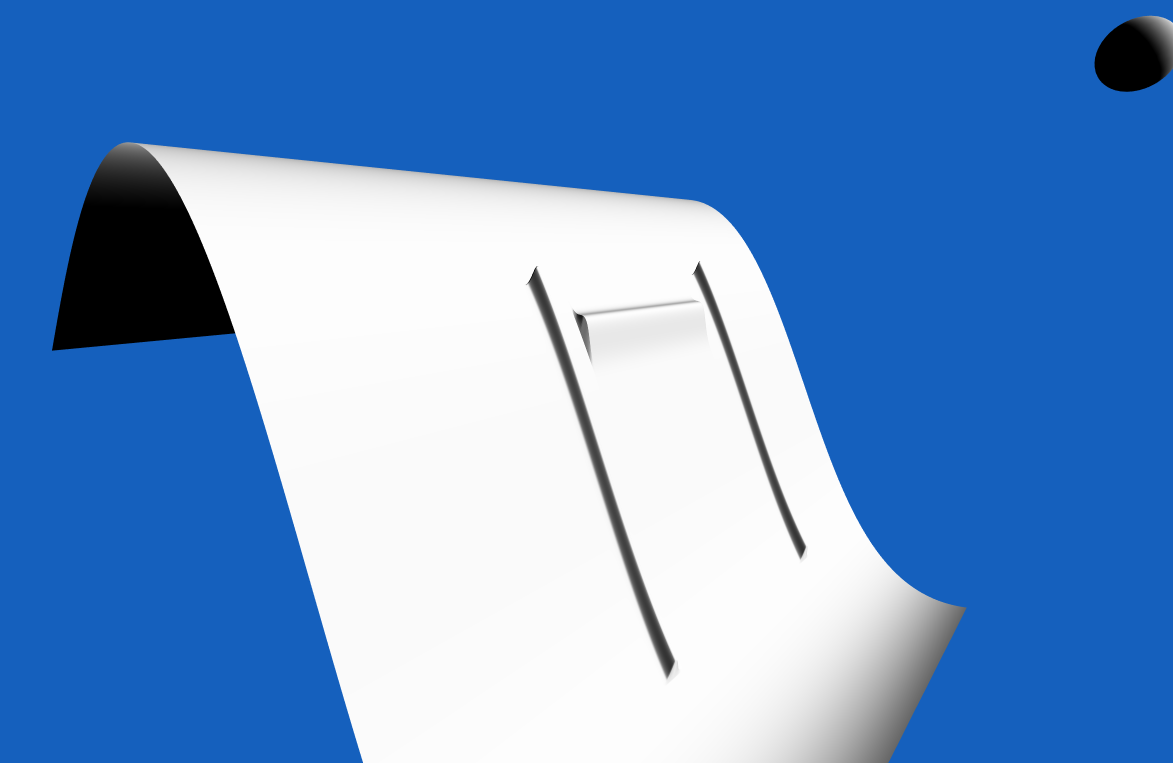
\includegraphics[width=0.4\textwidth]{Images/Essais/Essai_7_slint_East_0.png}
\end{tabular}
\subsubsection{Est, model 2}
\begin{tabular}{cc}
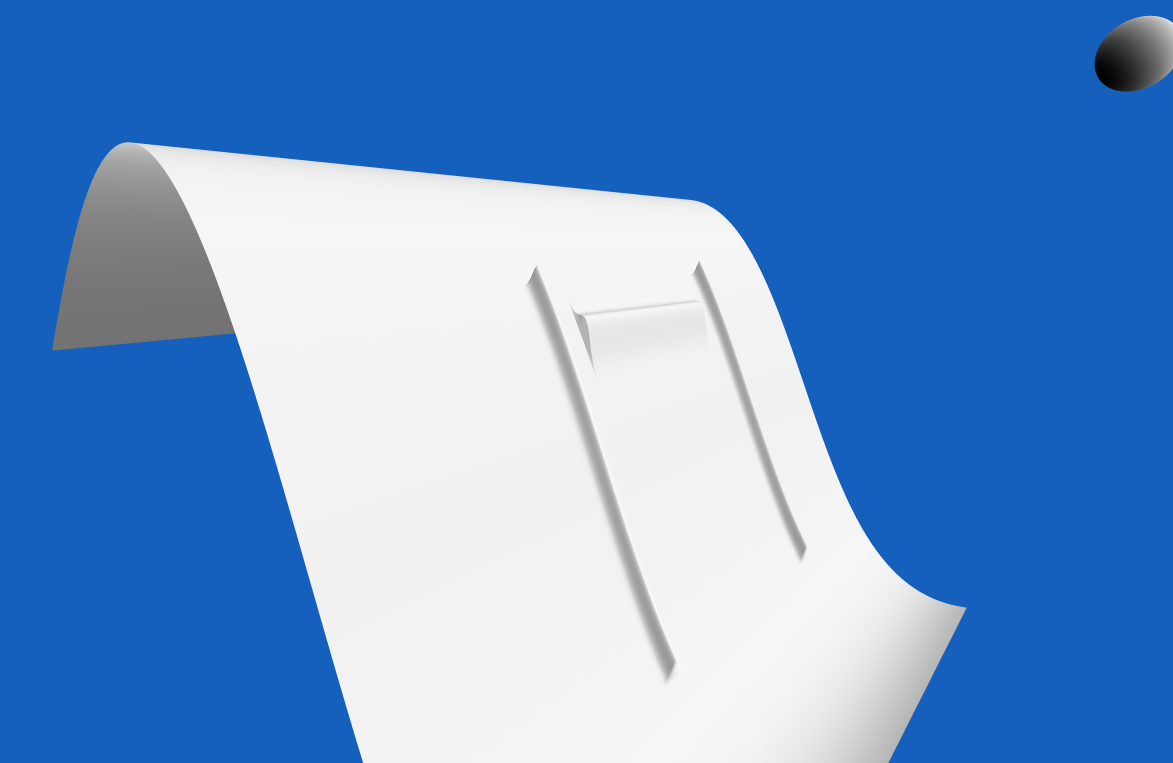
\includegraphics[width=0.4\textwidth]{Images/Essais/Essai_7_phong_East_1.png}
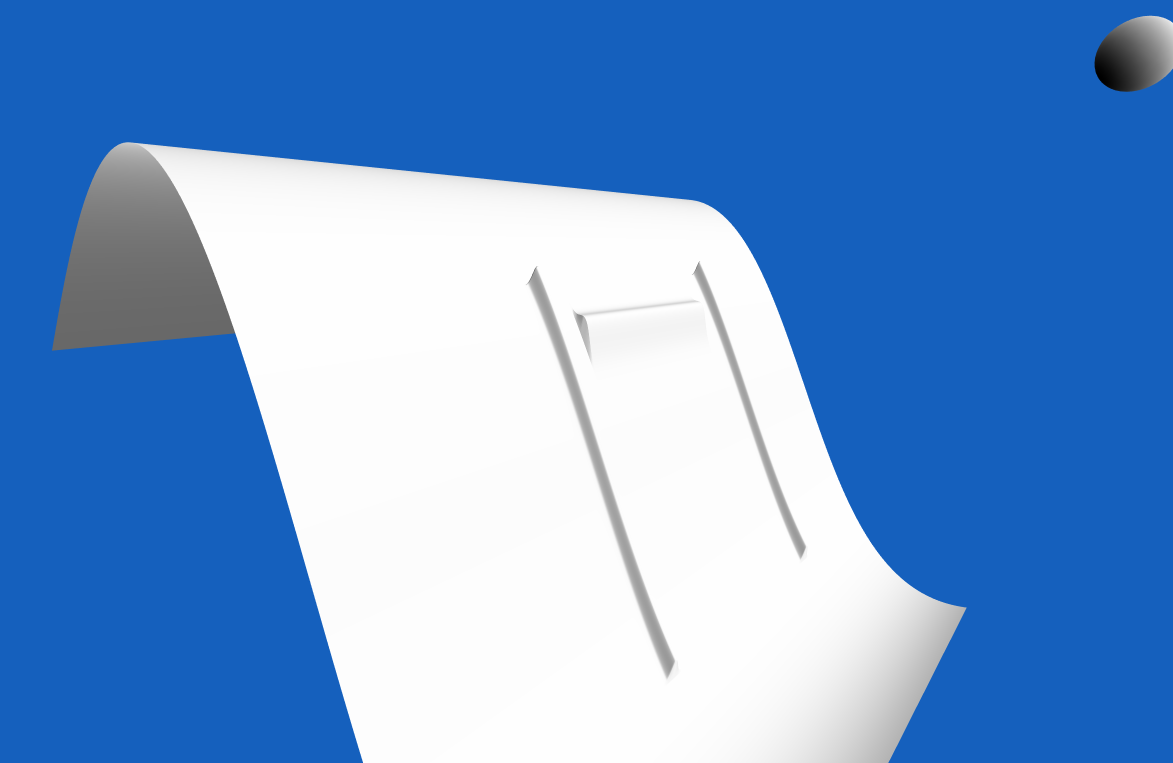
\includegraphics[width=0.4\textwidth]{Images/Essais/Essai_7_slint_East_1.png}
\end{tabular}
\subsubsection{Sud, model 1}
\begin{tabular}{cc}
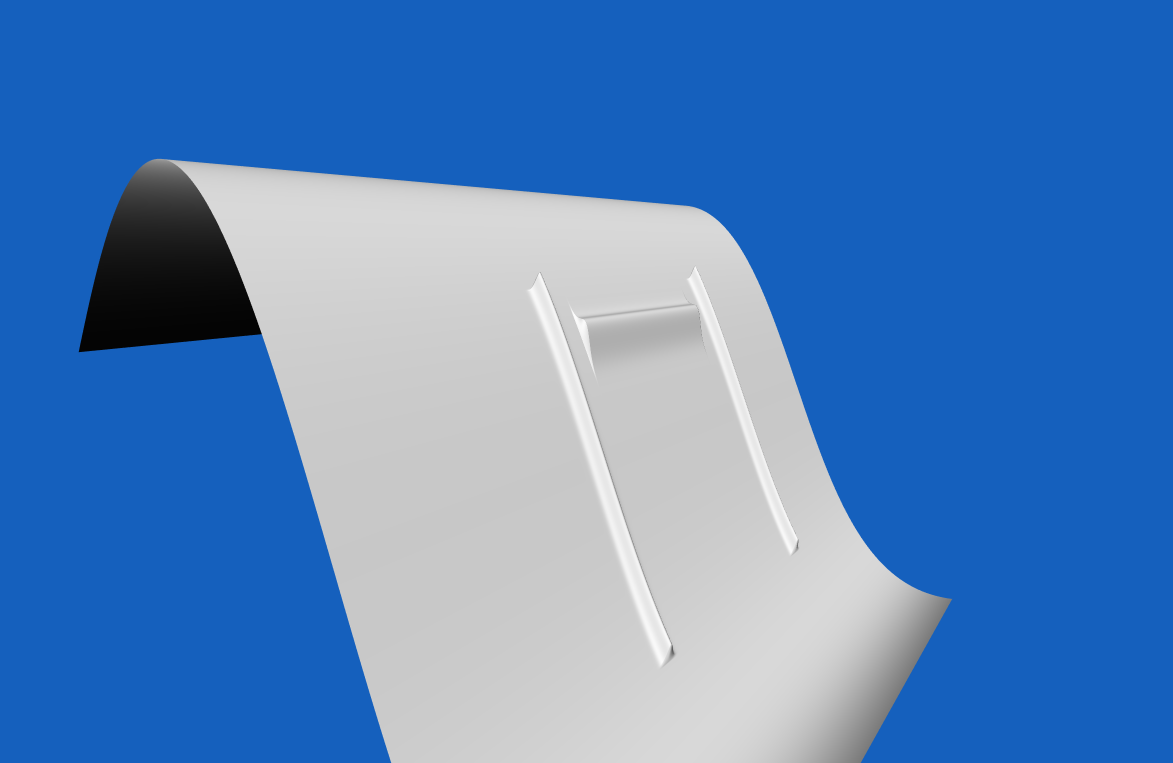
\includegraphics[width=0.4\textwidth]{Images/Essais/Essai_7_phong_South_0.png}
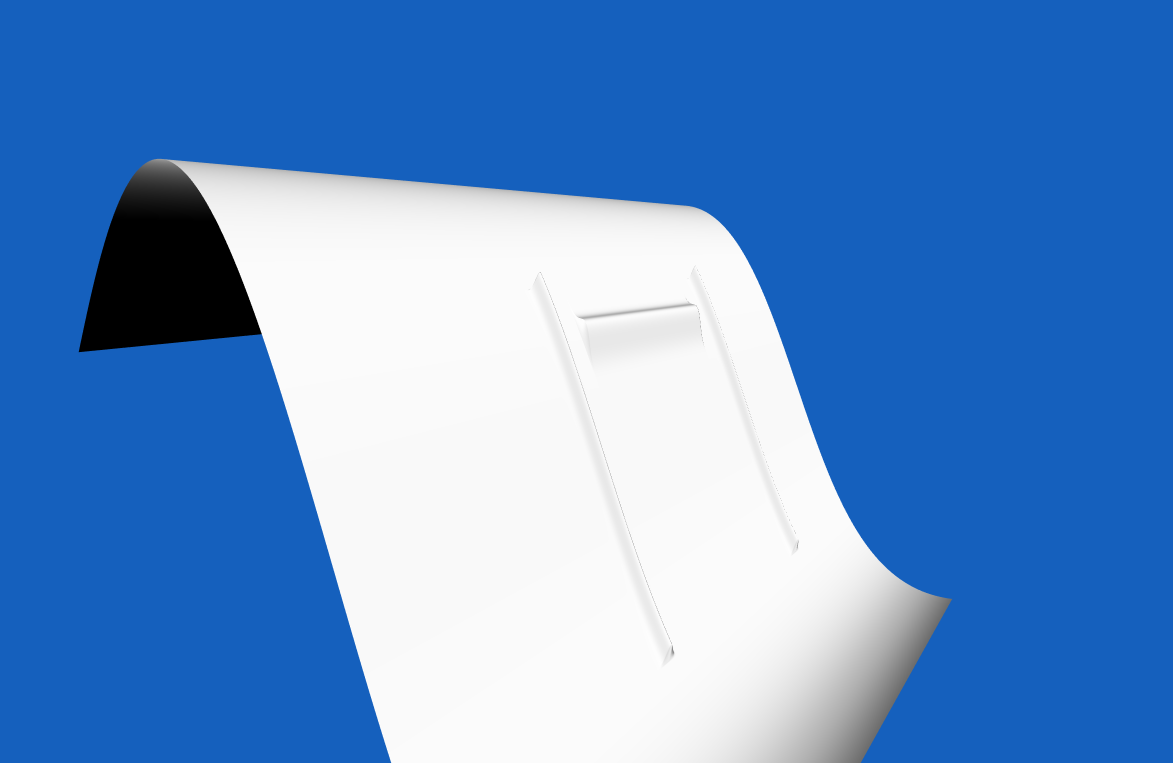
\includegraphics[width=0.4\textwidth]{Images/Essais/Essai_7_slint_South_0.png}
\end{tabular}
\subsubsection{Sud, model 2}
\begin{tabular}{cc}

\includegraphics[width=0.4\textwidth]{Images/Essais/Essai_7_phong_South_1.png}

\includegraphics[width=0.4\textwidth]{Images/Essais/Essai_7_slint_South_1.png}
\end{tabular}
\subsubsection{Ouest, model 1}
\begin{tabular}{cc}
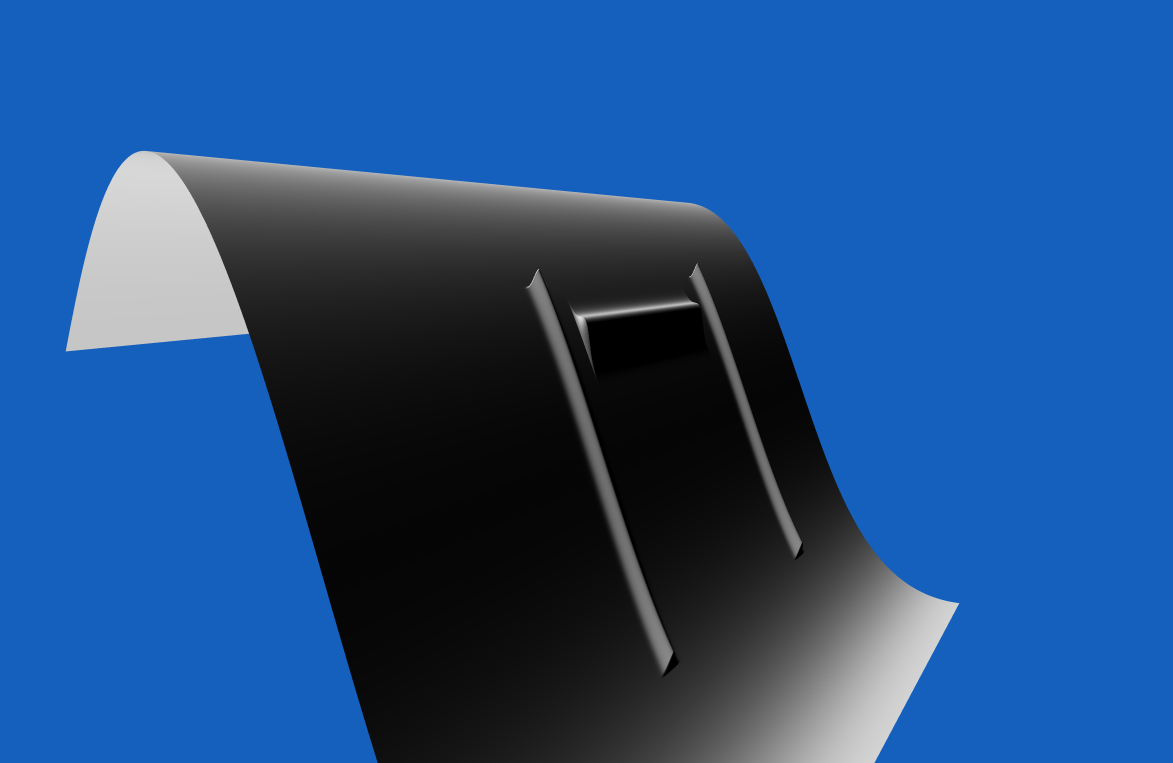
\includegraphics[width=0.4\textwidth]{Images/Essais/Essai_7_phong_West_0.png}
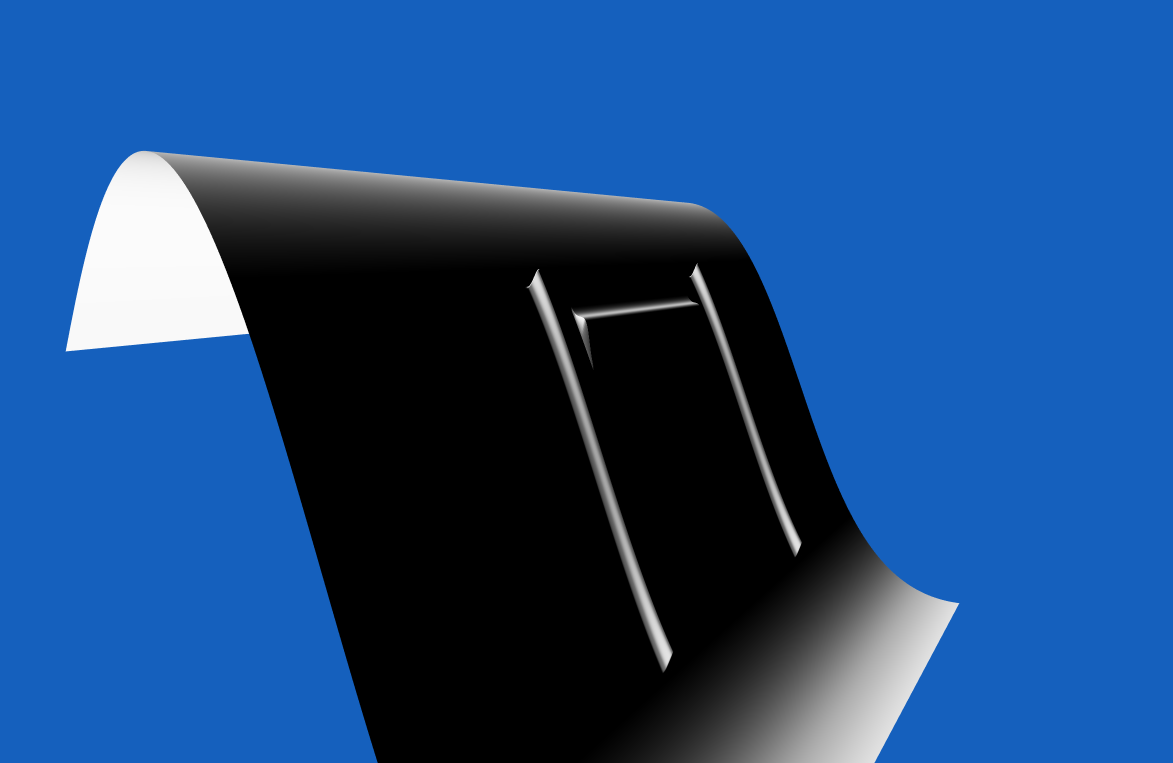
\includegraphics[width=0.4\textwidth]{Images/Essais/Essai_7_slint_West_0.png}
\end{tabular}
\subsubsection{Ouest, model 2}
\begin{tabular}{cc}
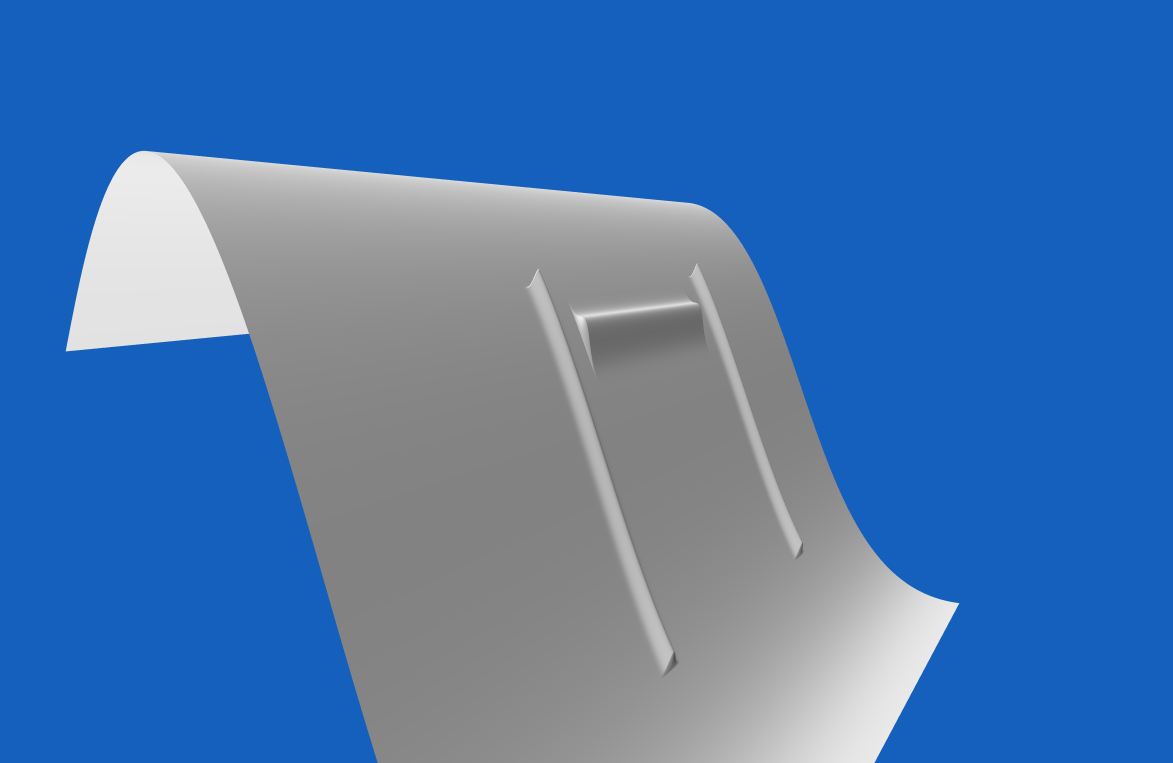
\includegraphics[width=0.4\textwidth]{Images/Essais/Essai_7_phong_West_1.png}
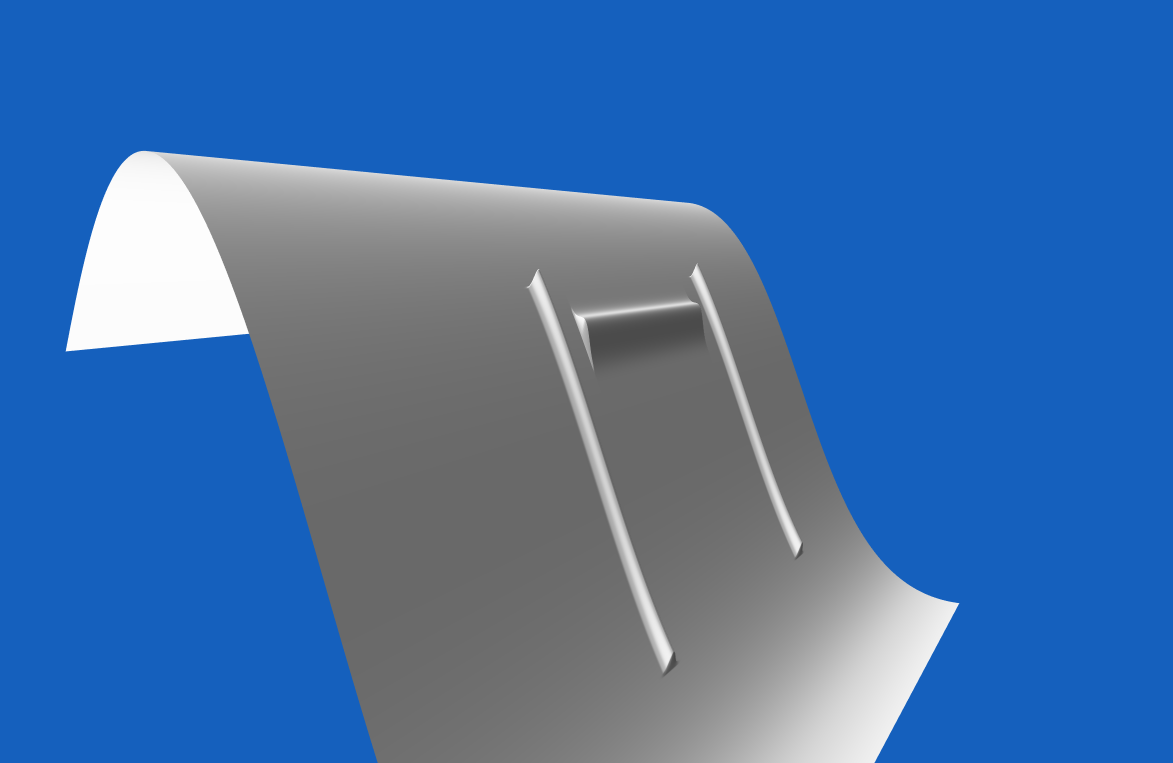
\includegraphics[width=0.4\textwidth]{Images/Essais/Essai_7_slint_West_1.png}
\end{tabular}





\subsection{Exploitation}
Pour chaque orientation , je sélectionne celle qui me semble la meilleur (mais ya un biais du fait que je veux que notre méthode soit sélectionné).\\
Donc ça donne :
\begin{itemize}
\item Nord : notre méthode , model 2.
\item Est : classique , model 2.
\item Sud : classique , model 1.
\item Ouest : notre méthode, model 2. 
\end{itemize} 

Pour astor : 
\begin{itemize}
\item Nord : notre méthode , model 2.
\item Est : classique , model 1.
\item Sud : classique , model 1.
\item Ouest : notre méthode, model 2. 
\end{itemize} 



Qu'est-ce qu'on peut en dire :
Avec notre méthode quand face observé fait face à la montagne , tout est blanc , car tout est éclairé et donc on voit rien.


\section{Essai 8-9}
\subsection{Principe}
On fait les screenshot plus proprement (automatisé) et on ajoute 2 bande en diagonale pour avoir une meilleur idée de ce qu'on veut. 
Ensuite pour l'essai 9 , on fait l'alignement de la lumière sur la carte flouté de manière ou aucune des petites features apparaissent.
Pour chaque section , de gauche à droite : phong , notre méthode , notre méthode + flou.  

\subsection{Résultats}
\subsubsection{Nord , model 1}
\begin{tabular}{cc}
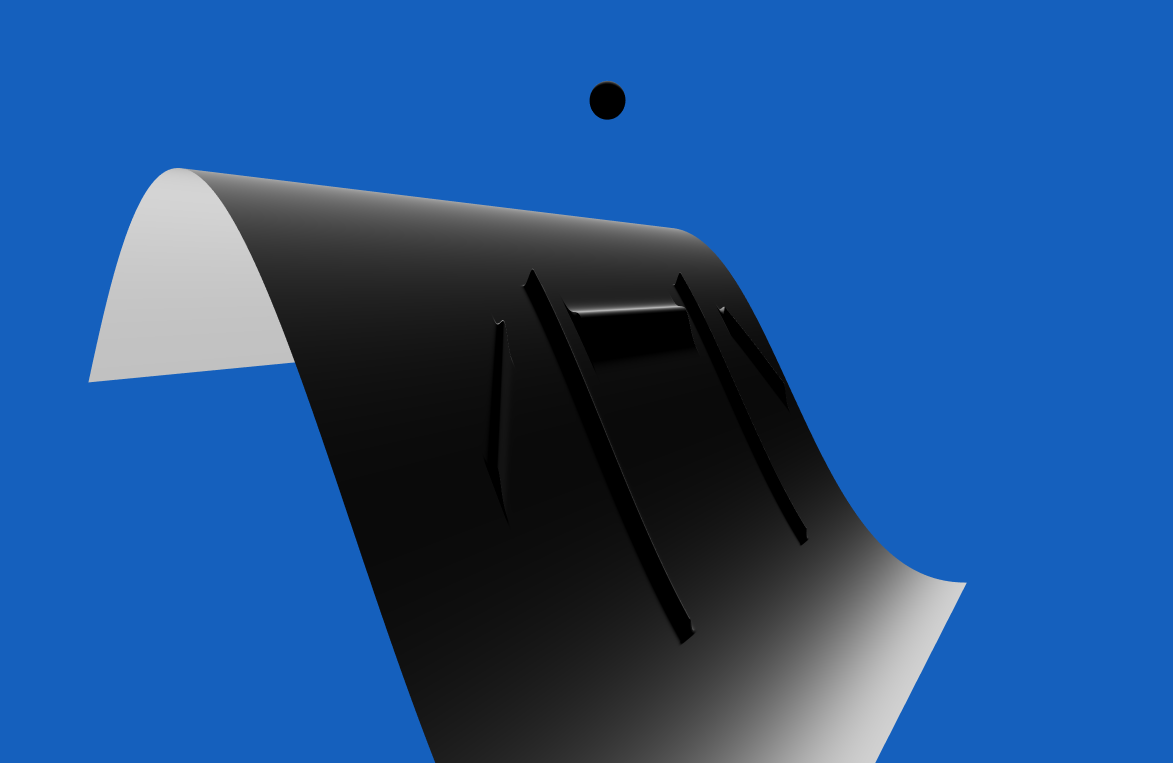
\includegraphics[width=0.3\textwidth]{Images/Essais/Essai_8_phong_North_0.png}
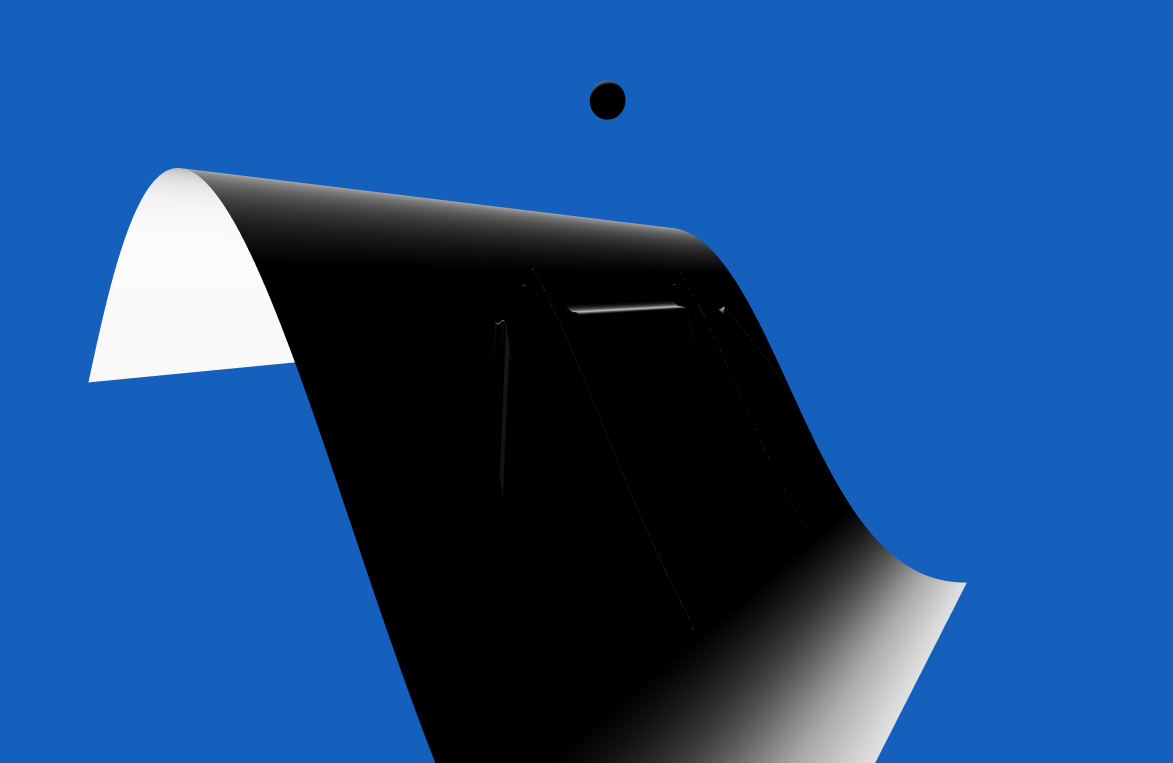
\includegraphics[width=0.3\textwidth]{Images/Essais/Essai_8_slint_North_0.png}
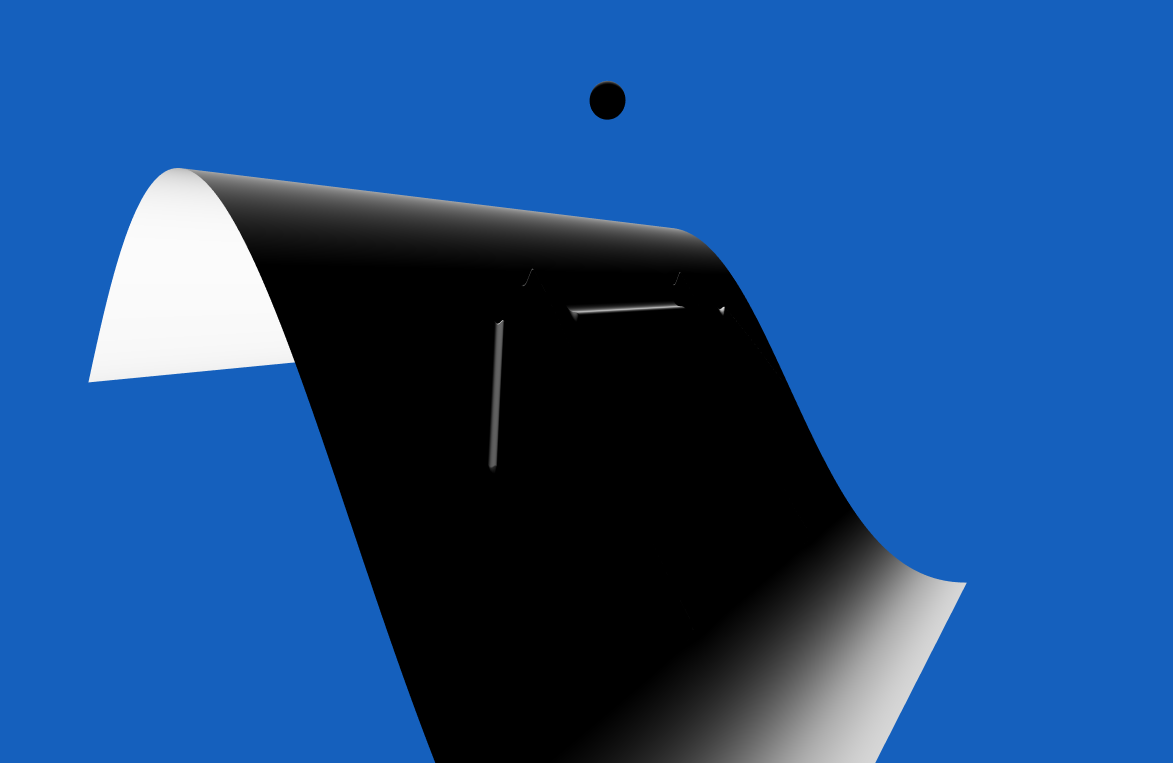
\includegraphics[width=0.3\textwidth]{Images/Essais/Essai_9_slint_North_0.png}
\end{tabular}


\subsubsection{Nord, model 2}
\begin{tabular}{cc}
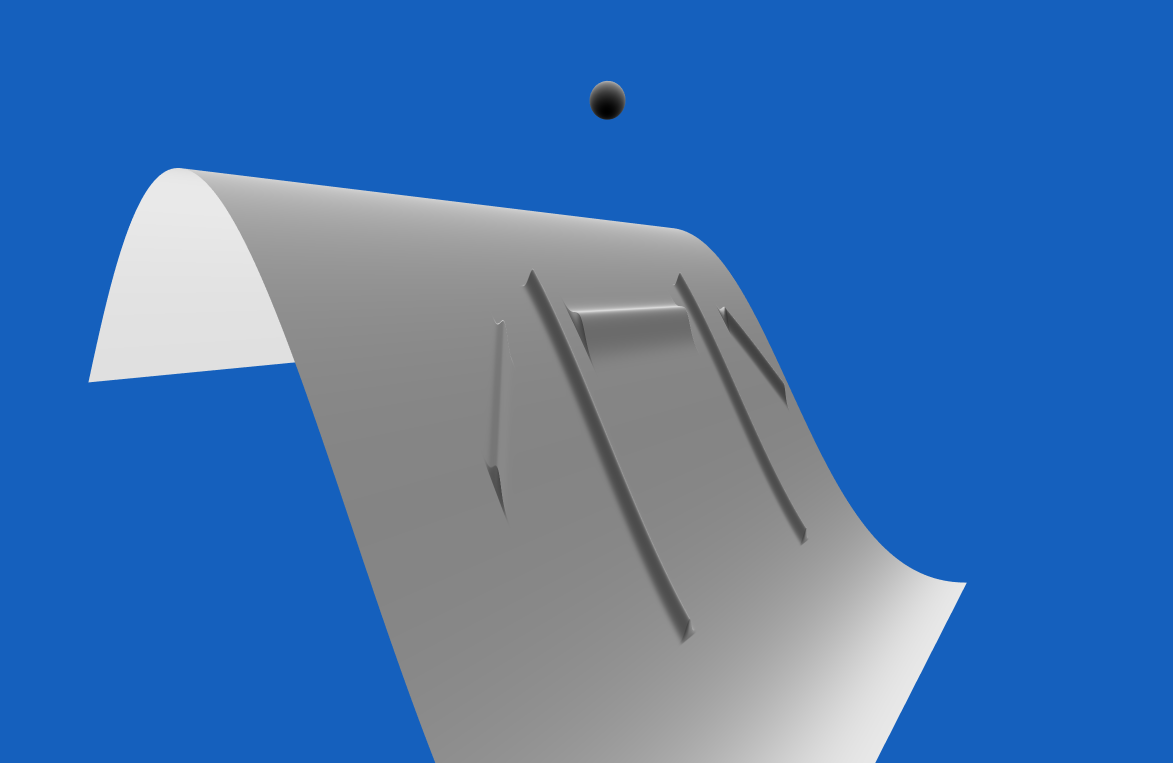
\includegraphics[width=0.3\textwidth]{Images/Essais/Essai_8_phong_North_1.png}
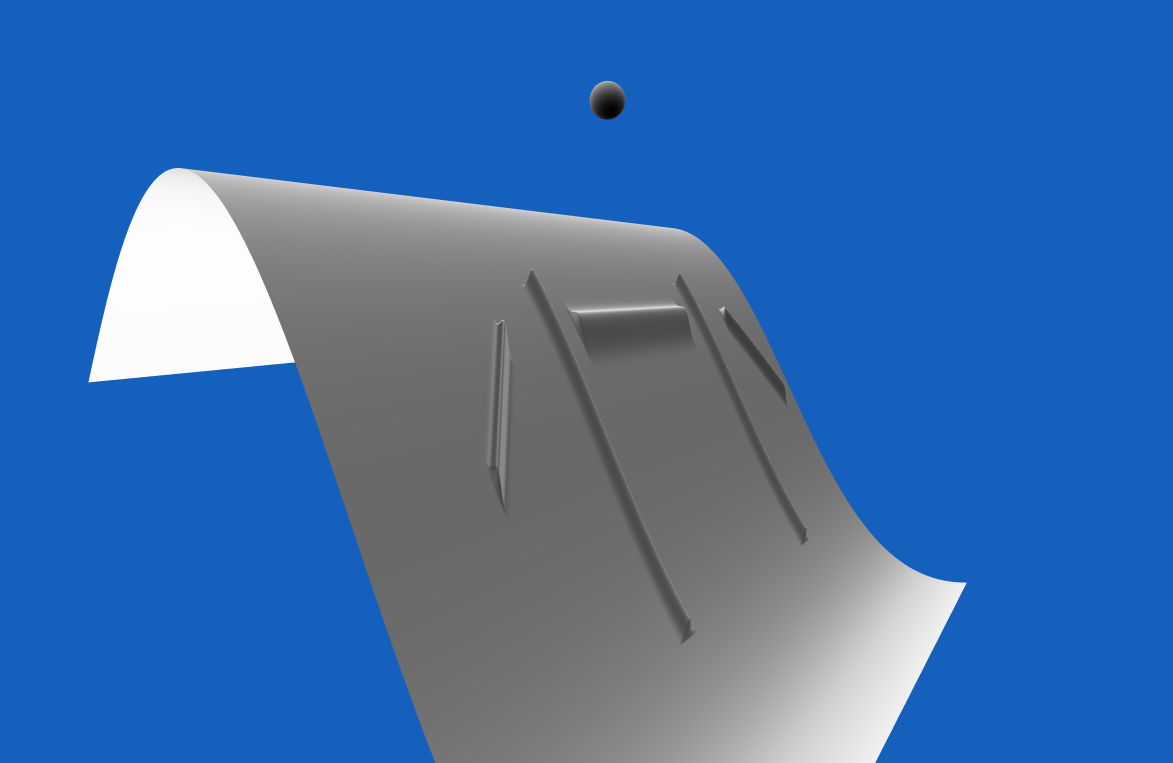
\includegraphics[width=0.3\textwidth]{Images/Essais/Essai_8_slint_North_1.png}
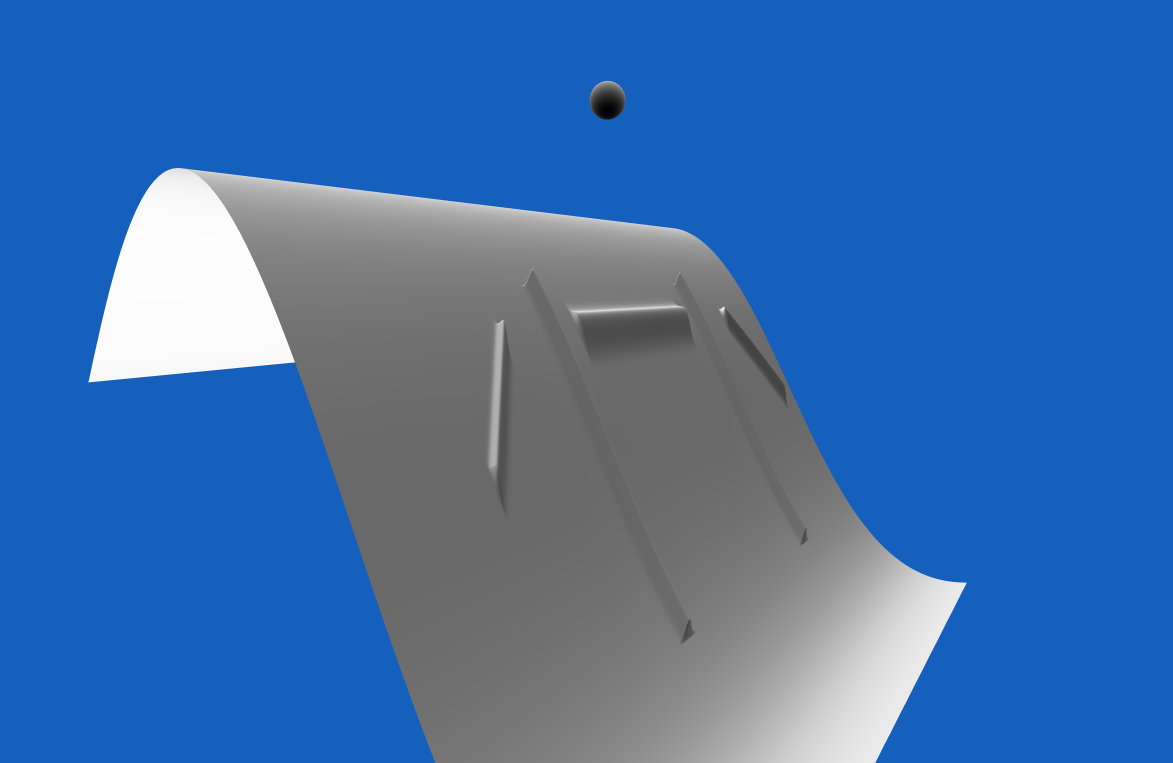
\includegraphics[width=0.3\textwidth]{Images/Essais/Essai_9_slint_North_1.png}
\end{tabular}

\subsubsection{Est, model 1}
\begin{tabular}{cc}
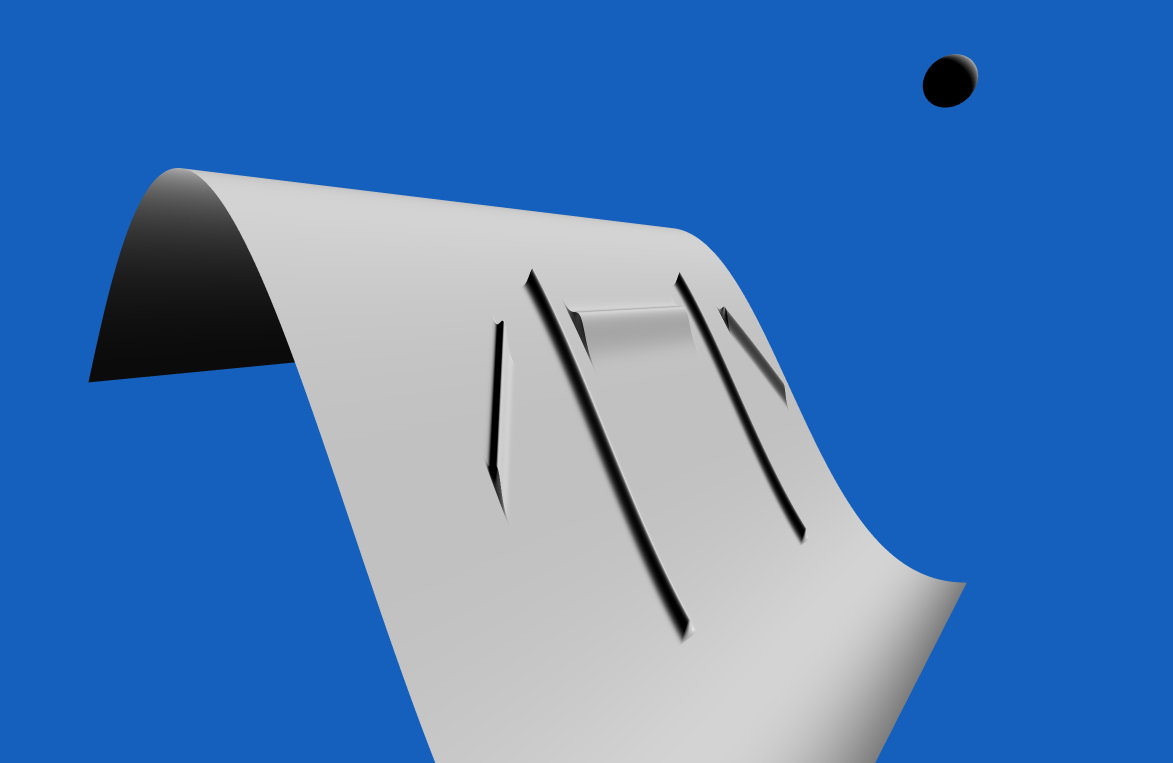
\includegraphics[width=0.3\textwidth]{Images/Essais/Essai_8_phong_East_0.png}
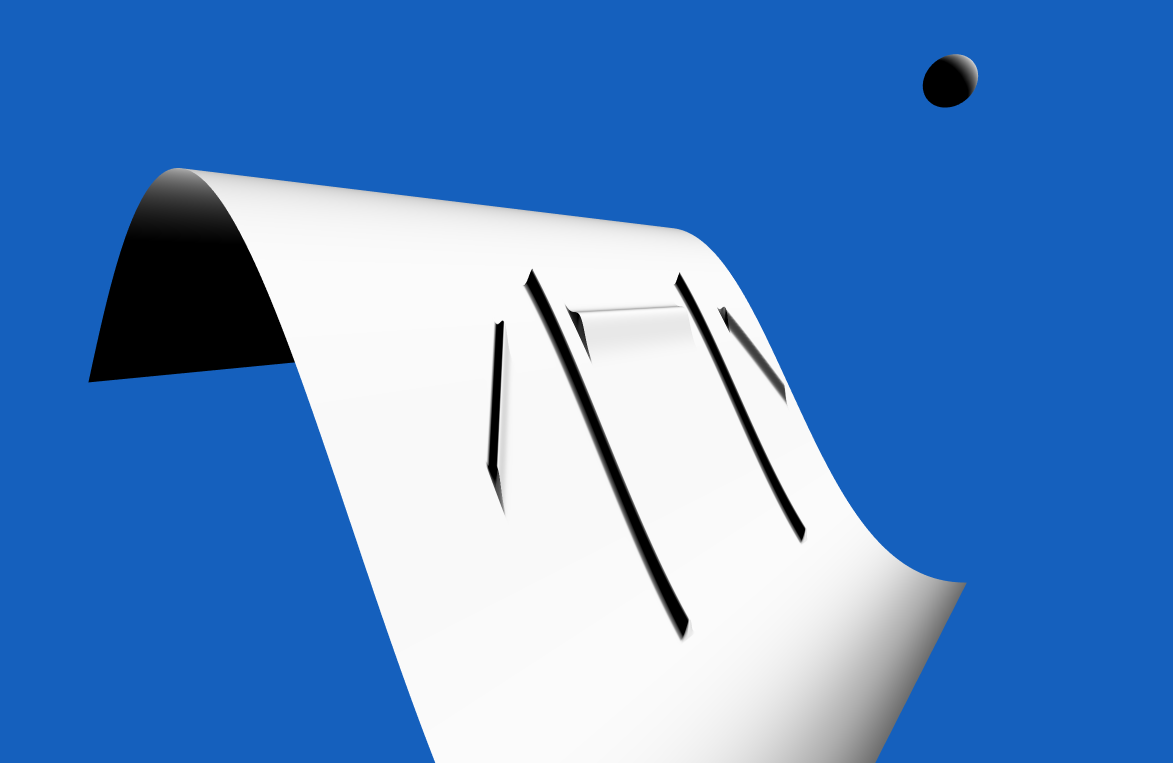
\includegraphics[width=0.3\textwidth]{Images/Essais/Essai_8_slint_East_0.png}
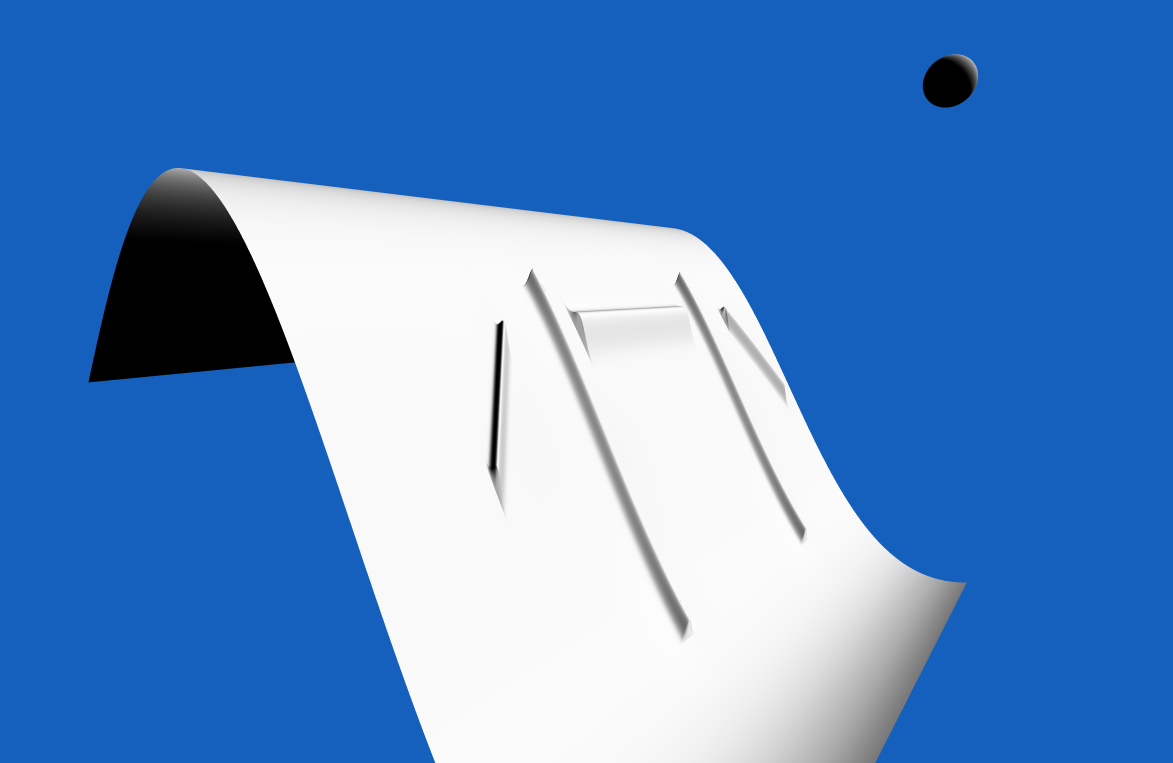
\includegraphics[width=0.3\textwidth]{Images/Essais/Essai_9_slint_East_0.png}
\end{tabular}
\subsubsection{Est, model 2}
\begin{tabular}{cc}
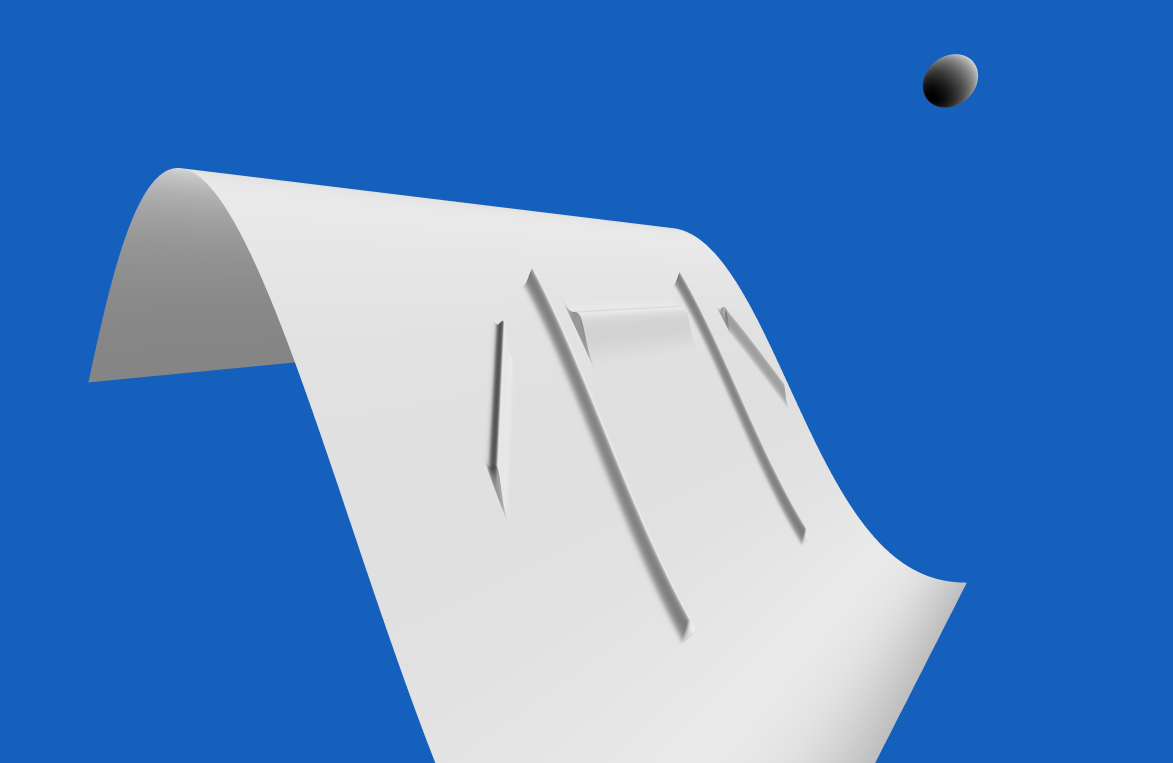
\includegraphics[width=0.3\textwidth]{Images/Essais/Essai_8_phong_East_1.png}
\includegraphics[width=0.3\textwidth]{Images/Essais/Essai_8_slint_East_1.png}
\includegraphics[width=0.3\textwidth]{Images/Essais/Essai_9_slint_East_1.png}

\end{tabular}
\subsubsection{Sud, model 1}
\begin{tabular}{cc}
\includegraphics[width=0.3\textwidth]{Images/Essais/Essai_8_phong_South_0.png}
\includegraphics[width=0.3\textwidth]{Images/Essais/Essai_8_slint_South_0.png}
\includegraphics[width=0.3\textwidth]{Images/Essais/Essai_9_slint_South_0.png}


\end{tabular}
\subsubsection{Sud, model 2}
\begin{tabular}{cc}
\includegraphics[width=0.3\textwidth]{Images/Essais/Essai_8_phong_South_1.png}
\includegraphics[width=0.3\textwidth]{Images/Essais/Essai_8_slint_South_1.png}
\includegraphics[width=0.3\textwidth]{Images/Essais/Essai_9_slint_South_1.png}

\end{tabular}
\subsubsection{Ouest, model 1}
\begin{tabular}{cc}
\includegraphics[width=0.3\textwidth]{Images/Essais/Essai_8_phong_West_0.png}
\includegraphics[width=0.3\textwidth]{Images/Essais/Essai_8_slint_West_0.png}
\includegraphics[width=0.3\textwidth]{Images/Essais/Essai_9_slint_West_0.png}

\end{tabular}
\subsubsection{Ouest, model 2}
\begin{tabular}{cc}
\includegraphics[width=0.3\textwidth]{Images/Essais/Essai_8_phong_West_1.png}
\includegraphics[width=0.3\textwidth]{Images/Essais/Essai_8_slint_West_1.png}
\includegraphics[width=0.3\textwidth]{Images/Essais/Essai_9_slint_West_1.png}

\end{tabular}

\section{Essai10}
\subsection{Principe}
On passe sur une montagne avec un bruit de perlin , c'est qui est beaucoup plus représentatif que des bosses fait à l'arrache.
\subsection{Résultats} 
\subsubsection{Nord , model 1}
\begin{tabular}{cc}
\includegraphics[width=0.4\textwidth]{Images/Essais/Essai_10_phong_North_0.png}
\includegraphics[width=0.4\textwidth]{Images/Essais/Essai_10_slint_North_0.png}
\end{tabular}

\subsubsection{Nord, model 2}
\begin{tabular}{cc}
\includegraphics[width=0.4\textwidth]{Images/Essais/Essai_10_phong_North_1.png}
\includegraphics[width=0.4\textwidth]{Images/Essais/Essai_10_slint_North_1.png}
\end{tabular}
\subsubsection{Est, model 1}
\begin{tabular}{cc}
\includegraphics[width=0.4\textwidth]{Images/Essais/Essai_10_phong_East_0.png}
\includegraphics[width=0.4\textwidth]{Images/Essais/Essai_10_slint_East_0.png}
\end{tabular}
\subsubsection{Est, model 2}
\begin{tabular}{cc}
\includegraphics[width=0.4\textwidth]{Images/Essais/Essai_10_phong_East_1.png}
\includegraphics[width=0.4\textwidth]{Images/Essais/Essai_10_slint_East_1.png}
\end{tabular}
\subsubsection{Sud, model 1}
\begin{tabular}{cc}
\includegraphics[width=0.4\textwidth]{Images/Essais/Essai_10_phong_South_0.png}
\includegraphics[width=0.4\textwidth]{Images/Essais/Essai_10_slint_South_0.png}
\end{tabular}
\subsubsection{Sud, model 2}
\begin{tabular}{cc}
\includegraphics[width=0.4\textwidth]{Images/Essais/Essai_10_phong_South_1.png}
\includegraphics[width=0.4\textwidth]{Images/Essais/Essai_10_slint_South_1.png}
\end{tabular}
\subsubsection{Ouest, model 1}
\begin{tabular}{cc}
\includegraphics[width=0.4\textwidth]{Images/Essais/Essai_10_phong_West_0.png}
\includegraphics[width=0.4\textwidth]{Images/Essais/Essai_10_slint_West_0.png}
\end{tabular}
\subsubsection{Ouest, model 2}
\begin{tabular}{cc}
\includegraphics[width=0.4\textwidth]{Images/Essais/Essai_10_phong_West_1.png}
\includegraphics[width=0.4\textwidth]{Images/Essais/Essai_10_slint_West_1.png}
\end{tabular}



\section{Essai 11}
\subsection{Principe}
En observant les images de l'essai d'avant une idée vient.
On obertse que avec notre méthode la face qui est à l'ombre est bien meilleur que le phong. L'idée est donc de faire en sorte d'etre toujours à l'ombre pour avec cette effet.
Pour ce faire , on utilise le multi echelle. On fait une passe sur une montagne très flouté pour n'avoir que les grande crete et on retourne la lumière si elle est dans le même sens que la normal. 
Et ensuite on faite une passe sur la carte normal et reprenant la lumière calculée à la passe d'avant et en alignant comme on le faisait avant. 
\subsection{Résultats}

\subsubsection{Nord , model 1}
\begin{tabular}{cc}
\includegraphics[width=0.4\textwidth]{Images/Essais/Essai_11_phong_North_0.png}
\includegraphics[width=0.4\textwidth]{Images/Essais/Essai_11_slint_North_0.png}
\end{tabular}

\subsubsection{Nord, model 2}
\begin{tabular}{cc}
\includegraphics[width=0.4\textwidth]{Images/Essais/Essai_11_phong_North_1.png}
\includegraphics[width=0.4\textwidth]{Images/Essais/Essai_11_slint_North_1.png}
\end{tabular}
\subsubsection{Est, model 1}
\begin{tabular}{cc}
\includegraphics[width=0.4\textwidth]{Images/Essais/Essai_11_phong_East_0.png}
\includegraphics[width=0.4\textwidth]{Images/Essais/Essai_11_slint_East_0.png}
\end{tabular}
\subsubsection{Est, model 2}
\begin{tabular}{cc}
\includegraphics[width=0.4\textwidth]{Images/Essais/Essai_11_phong_East_1.png}
\includegraphics[width=0.4\textwidth]{Images/Essais/Essai_11_slint_East_1.png}
\end{tabular}
\subsubsection{Sud, model 1}
\begin{tabular}{cc}
\includegraphics[width=0.4\textwidth]{Images/Essais/Essai_11_phong_South_0.png}
\includegraphics[width=0.4\textwidth]{Images/Essais/Essai_11_slint_South_0.png}
\end{tabular}
\subsubsection{Sud, model 2}
\begin{tabular}{cc}
\includegraphics[width=0.4\textwidth]{Images/Essais/Essai_11_phong_South_1.png}
\includegraphics[width=0.4\textwidth]{Images/Essais/Essai_11_slint_South_1.png}
\end{tabular}
\subsubsection{Ouest, model 1}
\begin{tabular}{cc}
\includegraphics[width=0.4\textwidth]{Images/Essais/Essai_11_phong_West_0.png}
\includegraphics[width=0.4\textwidth]{Images/Essais/Essai_11_slint_West_0.png}
\end{tabular}
\subsubsection{Ouest, model 2}
\begin{tabular}{cc}
\includegraphics[width=0.4\textwidth]{Images/Essais/Essai_11_phong_West_1.png}
\includegraphics[width=0.4\textwidth]{Images/Essais/Essai_11_slint_West_1.png}
\end{tabular}





\section{Essai 12}
\subsection{Principe}

On part sur une autre idée.
Dans un premier temps , on va mettre de coté la lumière et se concentrer sur les normales.
Dans cet essai, on a 2 version de la même heightMap , une flouté , l'autre non. 
On va creer une 3eme heightMap en soustrayant la non flouté à la flouté de manière a obtenir sur la 3eme uniquement les petites features en supprimant les grosses.
A partir de cette 3 eme heightMap, on calcule ses normales, on les applique directement sur le maillage et on calcule un Lambertien .



\subsection{Resultats}
A Gauche , le shading normal. A gauche le shading modifié. \\
\begin{tabular}{cc}
\includegraphics[width=0.4\textwidth]{Images/Essais/Essai_12_phong.png}
\includegraphics[width=0.4\textwidth]{Images/Essais/Essai_12_phong_editnormal.png}
\end{tabular}




\section{Essai 13}
\subsection{Principe}
On continu sur l'idée précédente et on rajoute l'orientation de la lumière. Il faut donc fusionner les informations entre les 2 échelles, la question est quel information faut-il fusionner et comment faut-il la fusionner ?
2 cas s'offre à nous : 
\begin{itemize}
\item L'angle de correction de chaque échelle.
\item Le diffu de chaque echelle.
\end{itemize} 

Dans cette essai , on s'intéresse à la fusion des angles.
Pour ce faire , on calcule les angles de correction comme avant (en alignant avec la pente et en multipliant par un smoothstep  et le norm de la pente (pour eviter toutes discontinuité). 
Et on fusionne en faisant une moyenne des 2 angles. On est sur les cercles trigonométrique , donc une moyenne arithmétique ne peux pas marcher. On utilise donc une autre formule : \\

Soit $y1$ et $y2$ les 2 angles de correction. 

\[y = \arctan\left(\frac{\sin(y_1)+\sin(y_2)}{2} , \frac{\cos(y_1)+\cos(y_2)}{2} \right)\]



\subsection{Résultats}
On a un probleme avec cette solution c'est que en faisant la moyenne, on efface certain features. \\
Map de l'angle Yaw corrigé , de gauche à droite, détaillé, flou , fusion.

\begin{tabular}{cc}
\includegraphics[width=0.3\textwidth]{Images/Essais/Essai_13_details.png}
\includegraphics[width=0.3\textwidth]{Images/Essais/Essai_13_flou.png}
\includegraphics[width=0.3\textwidth]{Images/Essais/Essai_13_fusion.png}
\end{tabular}

A gauche un cosing shading classic, à droite la fusion. \\
\begin{tabular}{cc}
\includegraphics[width=0.44\textwidth]{Images/Essais/Essai_13_phong_world.png}
\includegraphics[width=0.44\textwidth]{Images/Essais/Essai_13_fusion_world.png}
\end{tabular}

De plus , on a pas une différence très importante avec le phong classique car avec la fusion, la direction de lumière local se rapproche plus de la direction de la lumière global.
 



\section{Essai 14}
\subsection{Principe}
On test cette fois la fusion des diffus.
Pour ce faire , on fait juste une interpolation linéaire entre les 2 diffus ($d_1$ et $d_2$), avec un facteur $f$ de 0.5.
\[ d = d_1 *(1 - f) + d_2*f \]
  

\subsection{Résultats}

\begin{tabular}{cc}
\includegraphics[width=0.4\textwidth]{Images/Essais/Essai_14_details.png}&
\includegraphics[width=0.4\textwidth]{Images/Essais/Essai_14_flou.png} \\
\includegraphics[width=0.4\textwidth]{Images/Essais/Essai_14_fusion.png}&
\includegraphics[width=0.4\textwidth]{Images/Essais/Essai_14_phong.png}\\
\end{tabular}



Le résultats est plus proche de ce qu'on veut obtenir qu'avec le fusion de lumière. Il faut juste trouver un moyen de les fusions correctement.\\
Par contre, il y a 2 default. 
\begin{itemize}
\item Le flou décale un peu les crêtes et donc on a pas toujours une ombre marqué d'un coté et de l'autre de la crête 
\end{itemize}



\section{Essai 15}

\subsection{Principe}

On retravaille la fusion de diffus.\\
La question principale est : qu'est-ce qu'on veut obtenir ? \\
Il y a 2 aspect, la perception des détails et le style. \\
La perception des détails (shading): On veut voir le maximum de détails, c'est à dire qu'il faut un maximum de variation de couleur pour identifier les features. Aussi, on veut avoir des montagnes avec une face à l'ombre et une face éclairée.\\ 
Le style : Il faut quelque chose d'assez contrasté, nerveux. Où quand il y a une ombre ,elle soit marqué.

Du coup est-ce qu'on peut et est-ce qu'on doit séparer le style du shading ?
Si on sépare , ça voudrait dire que dans un premier temps , on fait un shading qui a pour but d'uniquement indiquer les variations du terrain. Et que dans un second temps on fait un cel-shading pour reproduire de style de Novat. Concrètement ça voudrait dire: est-ce que a partir d'uniquement le mix de diffus+ cel-shading fait à l'essai 14 permettrait de reproduire le style de novat ou alors c'est la combinaison des 2 diffus qui va permettre de faire ce style et que le cel-shading sert uniquement à rajouter de la couleur ? \\

Personnellement , je pense que la $1^{er}$ solution serai plus propre , afin d'avoir une séparation net mais elle sera de moins bonne qualité. Pour reproduire le style de Novat il est important d'avoir plusieurs information en même temps : si le point est dans l'ombre d'une montagne ou non et si le point est dans l'ombre d'une feature ou non. Or avec le mix, un point peut avoir la même couleur si il est dans l'ombre d'une montagne et si il est dans l'ombre d'une feature. Et donc ça semble difficilement rattrapable avec le cel-shading.\\
Du coup le 2eme cas semble plus facile et en théorie devrait donner de meilleur résultat.\\

Donc c'est ce qu'on essaye de faire dans cette essai.\\
Ce qu'on veut c'est quand le point est dans l'ombre d'une montagne et dans l'ombre d'une feature , qu'il soit plus noir que s'il était seulement dans l'ombre de la montagne. Et s'il est du coté eclairé de la feature mais toujours dans l'ombre de la montagne , qu'il soit plus sombre que si il était du coté éclairé de la montagne. Et inversement pour le coté éclairé de la montagne


Donc on résume : (D = détail, F = flou ) \\
\begin{tabular}{|c|c|c|}
  \hline
  F & D & R \\
  \hline
  N & N & N+ \\
  N & B & B+ \\
  B & N & N- \\
  B & B & B- \\
  \hline
\end{tabular}

Donc pour ce faire , on utilise la méthode overlay qui permet de augmenter les noir et les blancs en fonction de la couleur du flou. 

 

\[ Cd = 
\left\{
    \begin{array}{ll}
        1-2(1-D)(1-F)& \mbox{si } F > 0.5 \\
		2DF  & \mbox{sinon}				
    \end{array}
\right.
\]

Voici ça courbe : \\
\includegraphics[width=0.5\textwidth]{graphes/overlay_curve.png}

Ici il y a un problème c'est que quand le flou est à 0 ou à 1, on a plus aucune variation de couleur . Donc on remap le flou entre $[0.1 et 0.9]$ pour quand même avoir les petits détails.

\subsection{Resultats}

De gauche à droite et de haut en bas : lambertien classique, mix avec une facteur de 0.5, overlay et overlay. 


\begin{tabular}{cc}
\includegraphics[width=0.4\textwidth]{Images/Essais/Essai_15_phong.png}&
\includegraphics[width=0.4\textwidth]{Images/Essais/Essai_15_mix_05.png} \\
\includegraphics[width=0.4\textwidth]{Images/Essais/Essai_15_overlay.png}&
\includegraphics[width=0.4\textwidth]{Images/Essais/Essai_15_overlay_remap.png}\\
\end{tabular}


Le resultat est pas mal mais il est pas assez nerveux par rapport au style de novat. 


\section{Essai 16}
\subsection{Principe}
On reprend l'idée de l'essai 15 mais on change la formule. On utilise la formule d'aquarel d'ecrite dans le papier :Interactive watercolor rendering with temporal coherence and abstraction (\url{https://hal.inria.fr/inria-00510223/document})
Soit $f$ le diffus du  flou et $d$ le diffus du detail :
\[ C = d-(d-d^2)(f-1)\]

Et voici la courbe : \\
\includegraphics[width=0.5\textwidth]{graphes/watercolor_curve.png}

\section{Résultats}

Donc de gauche à droite et de haut en base : 
Le lambercien classique , le details, l'overlay remapé, et le watercolor.

\begin{tabular}{cc}
\includegraphics[width=0.4\textwidth]{Images/Essais/Essai_16_phong.png}&
\includegraphics[width=0.4\textwidth]{Images/Essais/Essai_16_details.png}\\
\includegraphics[width=0.4\textwidth]{Images/Essais/Essai_16_overlay_remap.png}&
\includegraphics[width=0.4\textwidth]{Images/Essais/Essai_16_watercolor.png}\\
\end{tabular}


 
 
 
 
\section{Formule}
On essaye de reformuler la formule proprement. Style exagerated Shading.

\begin{align*}
\theta_i &= (\vec{l}_{global},\vec{n}_{i_{xz}}) \\
\theta_i &= \theta_i * ||\vec{n}_{i_{xz}}|| * SmoothStep(T,\frac{\pi}{2},|\theta_i|)
\end{align*}
\[
\vec{l_i} = 
\begin{pmatrix}
X \\
Y \\
Z \\
\end{pmatrix}
=
\begin{pmatrix}
\cos \gamma  \cos \theta_i\\
\sin \gamma \\
\cos \gamma  \sin \theta_i \\
\end{pmatrix}
\] 

\[d_i = (\vec{l}_i \cdot{\vec{n}_i}) \]


\[ d = F(d_0,d_1) \]


Fonction fusion : \\
WaterColor :
\[ F(x,y) = x - (x -x^2)( 1-2y) \]
Overlay : 

\[F(x,y) = 
	\left\{
    \begin{array}{ll}
        1-2*(1-x)*(1-y) & \mbox{si } y > 0.5 \\
		2*x*y & \mbox{sinon}				
    \end{array}
\right.
\]


\[ c = C(d)  \]

C peut etre soit une multiplication avec une couleur Unie , soit une fonction de cel Shading , soit un waterColor avec une couleur donné, soit un colorMap. 






 




\section{Rapport et conclusion}
Version Final de l'ombrage : Voir le rapport du stage. \\
Couleur --> A Retravailler , essai avec l'altitude à faire \\
Ombres portées --> A Retravailler : Modifier l'elevation , trouver un filtre pour la forme (morphomath ou autre)
\\
Ombrage -> Essaie de multi echelle a faire. \\


\section{Essai 17}

On essaye de faire un xtoon.\\
Pour ce faire , on fait l'interpolation à la main en essayant d'être fidele au couleur qu'arthur nous a donné \\ 
Les couleur d'arthur (En x , le dégradé d'ombre, en y , le dégradé en fonction de l'altitude).\\

\includegraphics[width=0.4\textwidth]{Images/couleur_officiel_Novat.png}

Pour ce faire , on utilise le systeme HSV puis on convertie en RGB \\
H : En fonction de la hauteur , de 220 (basse altitude) 190 (haute altitude), \\
S : Fixe , 60 \\
V : Entre 0.5 et 1 en fonction de l'ombrage \\


\includegraphics[width=1.0\textwidth]{Images/Essais/Essai_17.png}

2eme paramétrisation : \\
$H = 220 - 25*hauteur$ \\
$S = 1 - Cd$ \\
$H = 0.4 + 0.6Cd$ \\
avec la hauteur en 0 et 1 , et Cd l'ombrage.

\includegraphics[width=1.0\textwidth]{Images/Essais/Essai_17_2.png}




\section{Essai 18}
Le multi echelle
Comme dit dans le rapport ça souleve 2 questions :
\begin{itemize}
\item Qu'est-ce que ça veut dire de faire un ombrage intermediaire
\item Comment les fusionner
\end{itemize}


Le probleme c'est que notre méthode de fusion est pas du tout adapter pour faire cela. Deplus <





\end{document}
